\documentclass[compress,xcolor=pdftex,dvipsnames,table]{beamer}

\usetheme{SimonFraser}
\usecolortheme{OfficialSimonFraser}
\usepackage{graphicx}
\usepackage{multimedia}
\usepackage{hyperref}
\hypersetup{colorlinks=true}
\hypersetup{bookmarks=false}

%
% define logo, usually either D0 or SFU
%
\title{MVA Status Update (lephad and hadhad)}
%\subtitle{I have no subtitle}
%\institute[SFU]{Simon Fraser University}
\author[Andres,Michel,Noel,Dugan]{Noel~Dawe, Andres~Tanasijczuk, Michel~Trottier-McDonald, Dugan~O'Neil}
\date[September 13, 2012]{September 13, 2012}
%\titlegraphic{
%\includegraphics[width=0.9\textwidth]{figures/group.png}
%}
% add logo to bottom right corner of each page
%\logo{\includegraphics[height=1.25cm]{figures/SFUcrest.jpg}}
% turn navigation symbols off
\beamerboxesdeclarecolorscheme{alert}{red}{red!15!averagebackgroundcolor}
\usebeamercolor[bg]{author}
\setbeamertemplate{navigation symbols}{}
%%%%
\def \et {E_{T}}
\def  \met {\not\!\!\et }
\newcommand{\greenchk}{\textcolor{ForestGreen}{$\checkmark$}}
\newcommand{\redX}{\textcolor{red}{X}}

%%%%

\begin{document}

\frame[plain]{\titlepage}

%%%
%%%
\frame{
\frametitle{Introduction/Reminder}

\begin{itemize}

\item This is an update of the analysis presented in the \href{https://indico.cern.ch/getFile.py/access?contribId=2&resId=0&materialId=slides&confId=158248}{August 2 HSG4 meeting}. 2011 re-analysis with BDTs.

\item Basic strategy, variable lists, etc. have not changed. Several
  improvements have been made to systematic uncertainty treatment,
  inclusion of lep+had triggers, embedding for hadhad, etc.

\item Variables were well-modelled and BDT control regions look nice!

\item At 125GeV, lephad expectation = $2.4*$SM (3.1 cut-based), hadhad
  expectation = $3.0*$SM (3.7 cut-based).

\item Changes have brought improved sensitivity, and a much shorter
  list of caveats.

\item Detailed ($>100$ page) note continues to be developed in
  \href{https://svnweb.cern.ch/trac/atlasphys/browser/Physics/Higgs/HSG4/ReOptimized2011/SM_MVA_HadHad_ReOptimized2011}{hadhad
    space}.

\end{itemize}

}

%%%
%%%
\frame{
\frametitle{Reminder: Analysis Strategy}

\begin{itemize}

\item Cut based analyses use a variety of categories (VBF, boosted,
  etc.) with relatively tight cuts to achieve best sensitivity.

\item The MVA approach defines the categories in a looser way and for
  a different reason. Distinct topological categories have different
  background compositions and may need different variable lists.

\item In defining categories, lephad and hadhad can be identical, but
  variable lists should be different.

\item Provide an approach, description, etc. which is as integrated as possible:
\begin{itemize}

\item BDTs are employed in each channel in the same categories. 

\item Validation is performed in the same way, common control regions where possible.

\item Final distribution for limit-setting is the BDT output in a mass (MMC) window (110-150GeV).

\end{itemize}

\end{itemize}

}

%%%
%%%
\frame{
\frametitle{Reminder: Categories}

\begin{itemize}

\item In each channel define three categories defined by number and $p_T$ of jets:
\begin{itemize}
 \item VBF: 2-3 jets, $p_T(j1)>50$~GeV, $p_T(j2)>30$~GeV 
 \item Boosted: not VBF but 1-3 jet, $p_T(j1)>50$~GeV 
 \item ggF: not VBF, not Boosted
\end{itemize}

\item Better stats in these categories than tighter approach, better for training, testing. 
\item Allows more phase-space for optimization.

\end{itemize}

}

%%%
%%%
\frame{
\frametitle{Reminder: Validation}

\begin{itemize}

\item In this analysis it is key to do validation of variable modelling in at least two ways (after checking basic kinematics, etc. for obvious issues):
\begin{enumerate}
 \item Are the input variables to the BDT well modeled in each channel and category?
 \item Is the combination of these input variables, the BDT score itself, well-modeled?
\end{enumerate}

\item The first one can be checked easily in each channel and category. The categorization is loose, no signal will be seen.

\item For the second, define signal free control regions and plot the BDT score in each. For example:
\begin{itemize}
\item Mass Sideband control region: $M_{\tau\tau}<110$GeV OR $M_{\tau\tau}>150$GeV
\item $Z$-rich control region (lephad): $M_{\tau\tau}<100$GeV, $m_T<40$GeV
\item $W$-rich control region (lephad): $M_T>70$GeV
\end{itemize}

\end{itemize}

}

%%%
%%%
\frame{
\frametitle{Previously Planned Improvements}

\begin{itemize}

\item Planned lephad improvements:
\begin{itemize}
 \item Adopt improved overlap removal from cut-based. (adopted in electrons).
 \item Add lepton+hadron triggers. (done)
 \item Fix JER systematics. (done) 
 \item Test alternate Z training samples, adopt embedding
   samples. (tests performed, embedding not used)
\end{itemize}

\item Planned hadhad improvements:
\begin{itemize}
 \item Use of embedding samples (done)
 \item Add uncertainty on continuous TauID score. (done)
\end{itemize}

\item General: add shape dependent theory uncertainty. First pass
  complete (see \href{https://indico.cern.ch/getFile.py/access?contribId=2&resId=0&materialId=slides&confId=186213}{slides}), but not included in limits shown
  today. % Theory uncertainty still under discussion.

\item Systematics: background normalization
  uncertainties added in both channels. Minor
  systematics updated to latest values.
\end{itemize}

}

%%%
\frame{
\frametitle{Lephad Analysis - other changes}

\begin{itemize}

\item Despite the good modelling shown previously, there were bugs in
  applying lepton corrections. Fixed.

\item Some categories or control regions showed bad modelling for $\Delta
  R(\ell,\tau)>3.5$. Cut applied.

\item Electron $p_T$ (and $\eta$) spectrum also had a strange shape in
  the boosted category. Bias in QCD model. Changed shape used to
  SS-isolated (from OS-not-Isolated). Fixed.

\item $MET>20$GeV cut added after training (to preserve training stats).

\item We now see no significant issues in the 1200-ish control plots
  we regularly make in lephad (see extra slides attached to the agenda).

\end{itemize}

}

%%%
\frame{
\frametitle{Lephad Analysis - VBF(e) Discriminating Variables}

\begin{columns}
\column{0.3\textwidth}
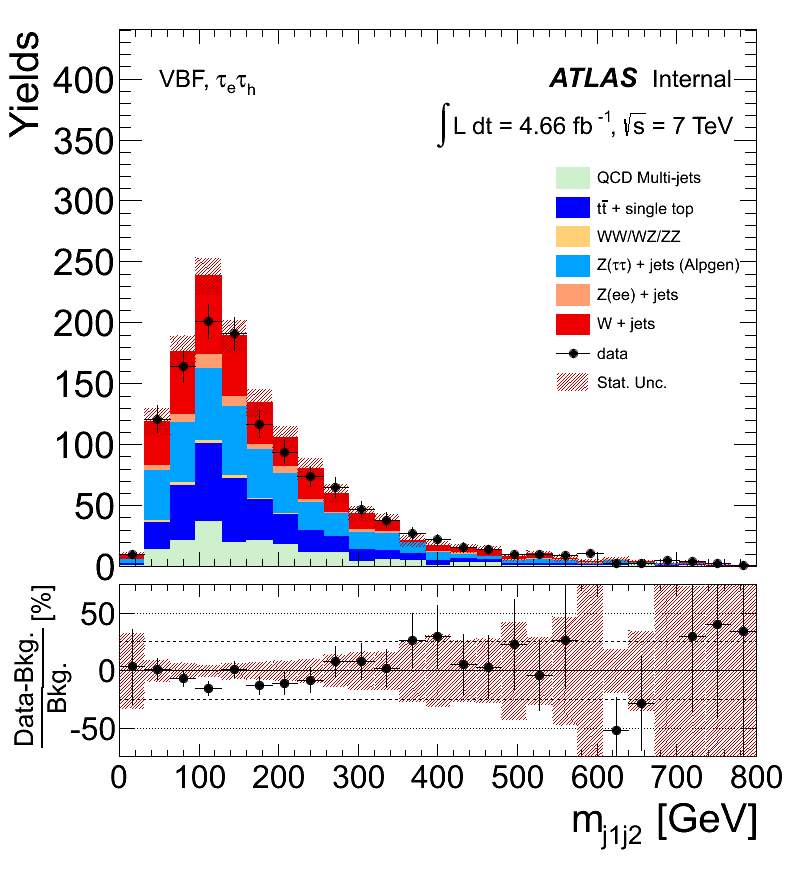
\includegraphics[width=\textwidth]{figures/lephad/e_mass_j1_j2_VBF_sig.png}\\
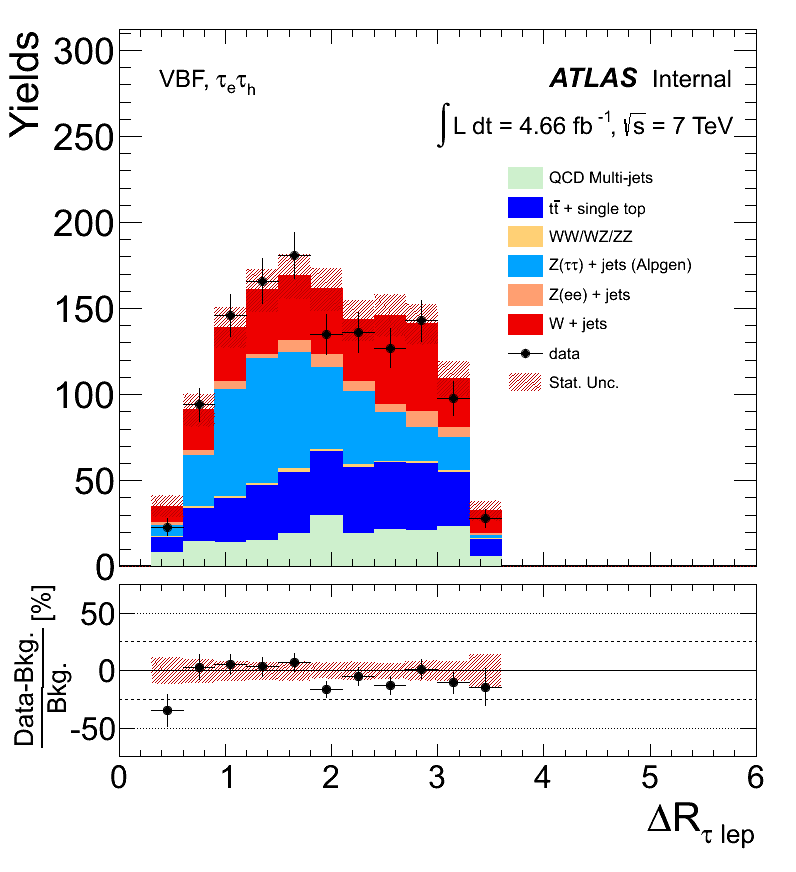
\includegraphics[width=\textwidth]{figures/lephad/e_dr_tau_lep_VBF_sig.png}
\column{0.3\textwidth}
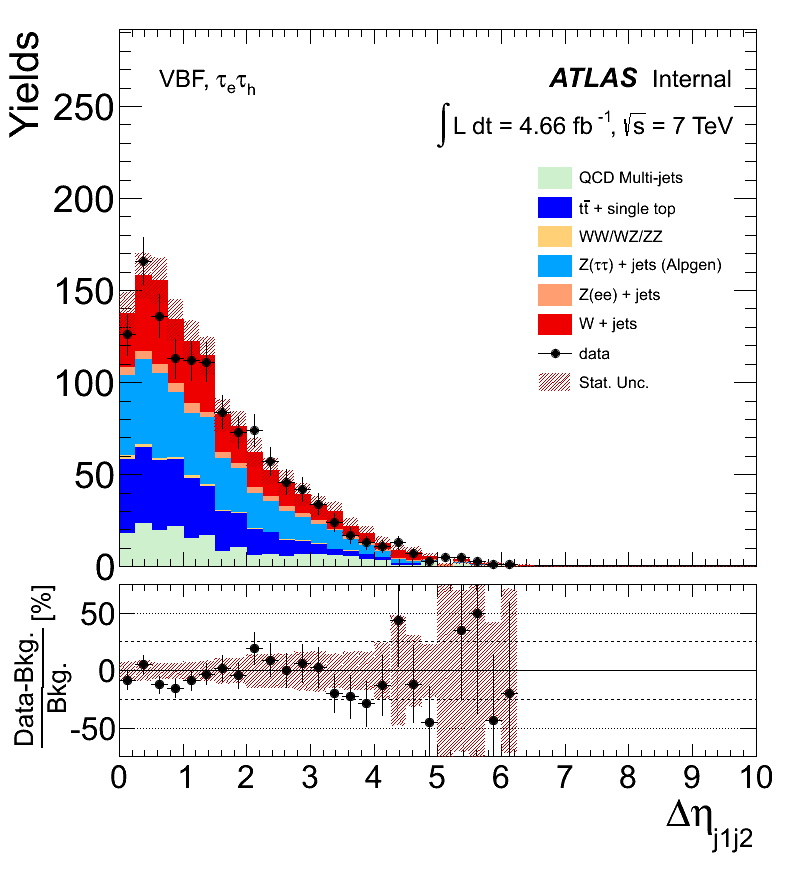
\includegraphics[width=\textwidth]{figures/lephad/e_eta_delta_j1_j2_VBF_sig.png}\\
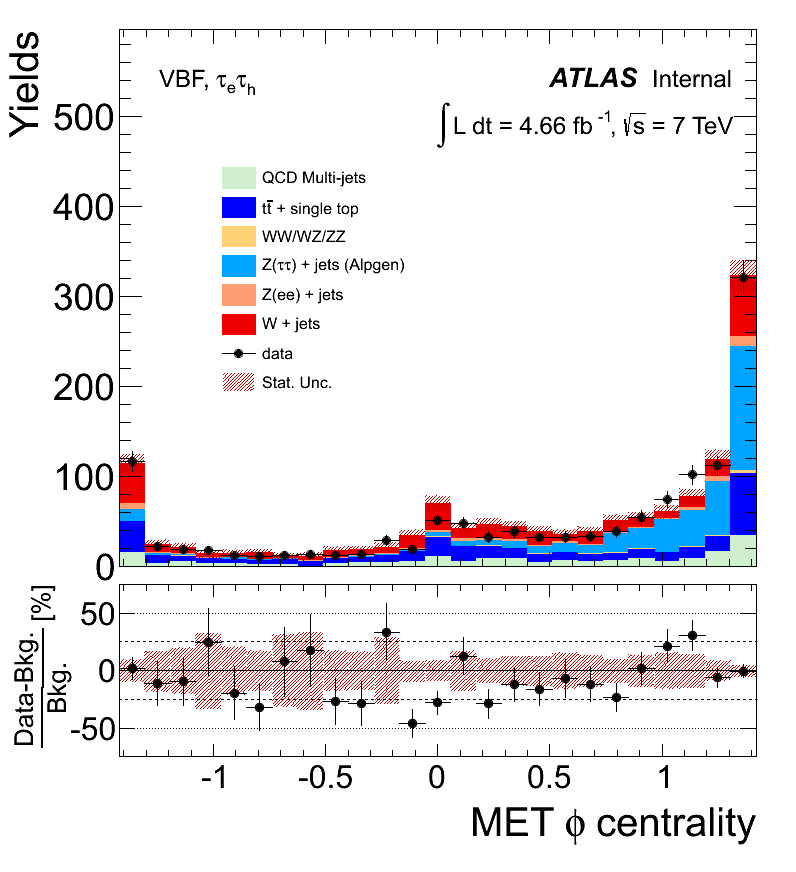
\includegraphics[width=\textwidth]{figures/lephad/e_met_phi_centrality_VBF_sig.png}
\column{0.3\textwidth}
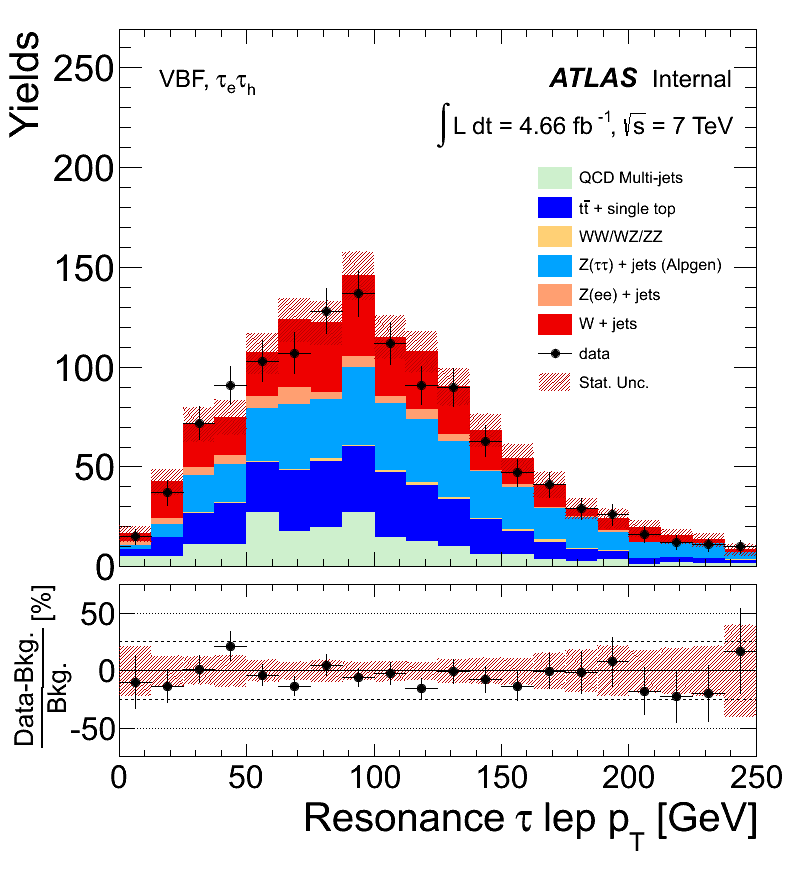
\includegraphics[width=\textwidth]{figures/lephad/e_resonance_pt_tau_lep_VBF_sig.png}\\
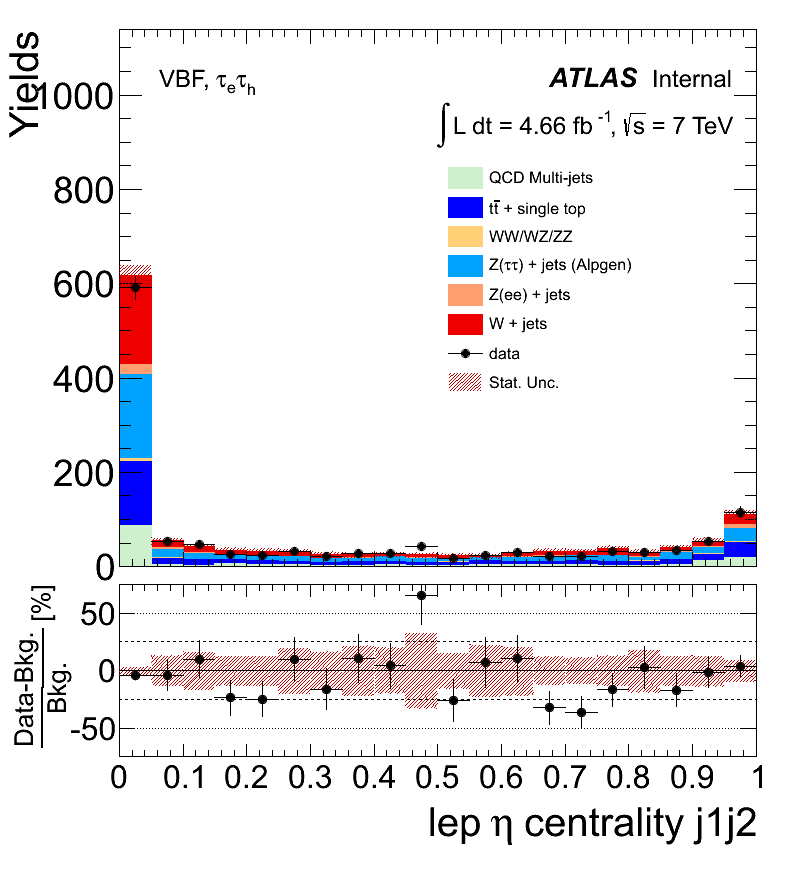
\includegraphics[width=\textwidth]{figures/lephad/e_lep_centrality_j1_j2_VBF_sig.png}
\end{columns}

}

%%%
\frame{
\frametitle{Lephad Analysis - Boosted($\mu$) Discriminating Variables}

\begin{columns}
\column{0.3\textwidth}
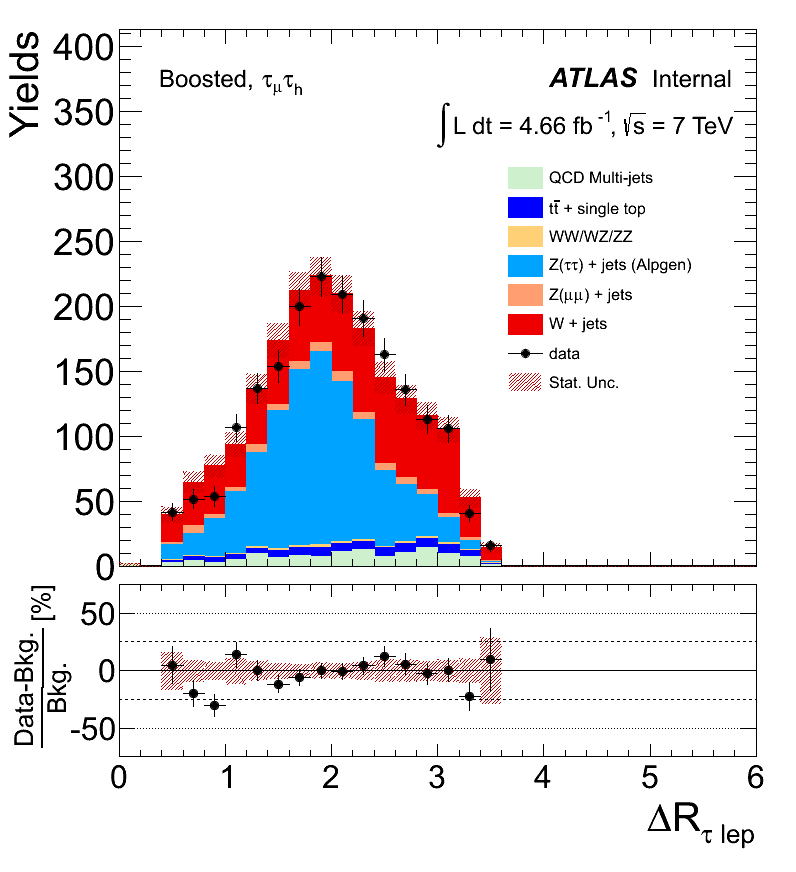
\includegraphics[width=\textwidth]{figures/lephad/mu_dr_tau_lep_boosted_sig.png}\\
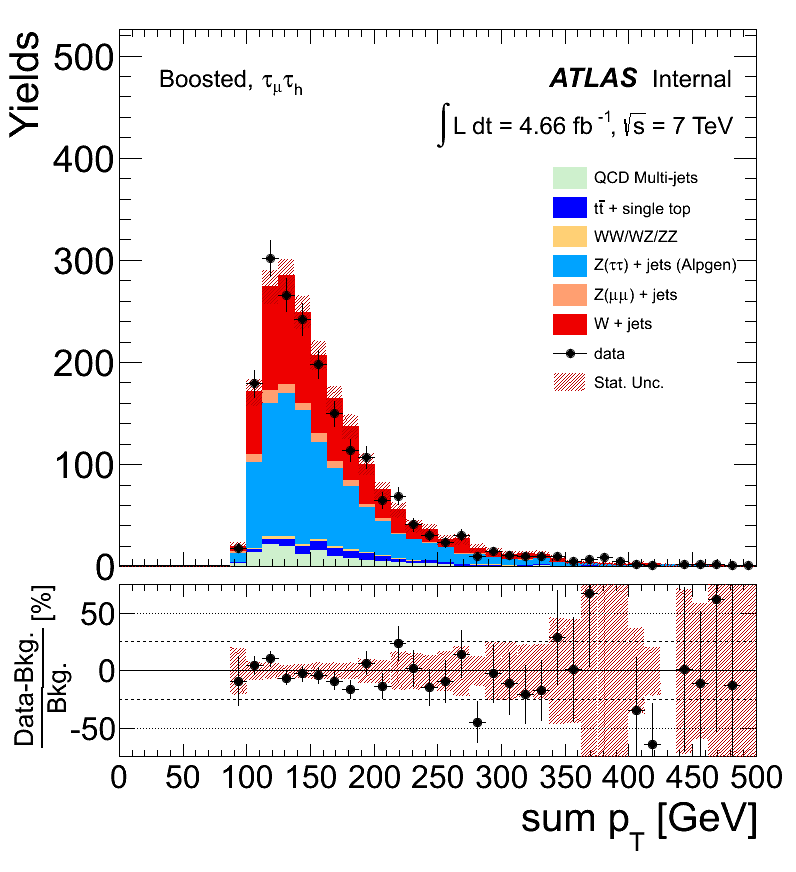
\includegraphics[width=\textwidth]{figures/lephad/mu_sumPt_boosted_sig.png}
\column{0.3\textwidth}
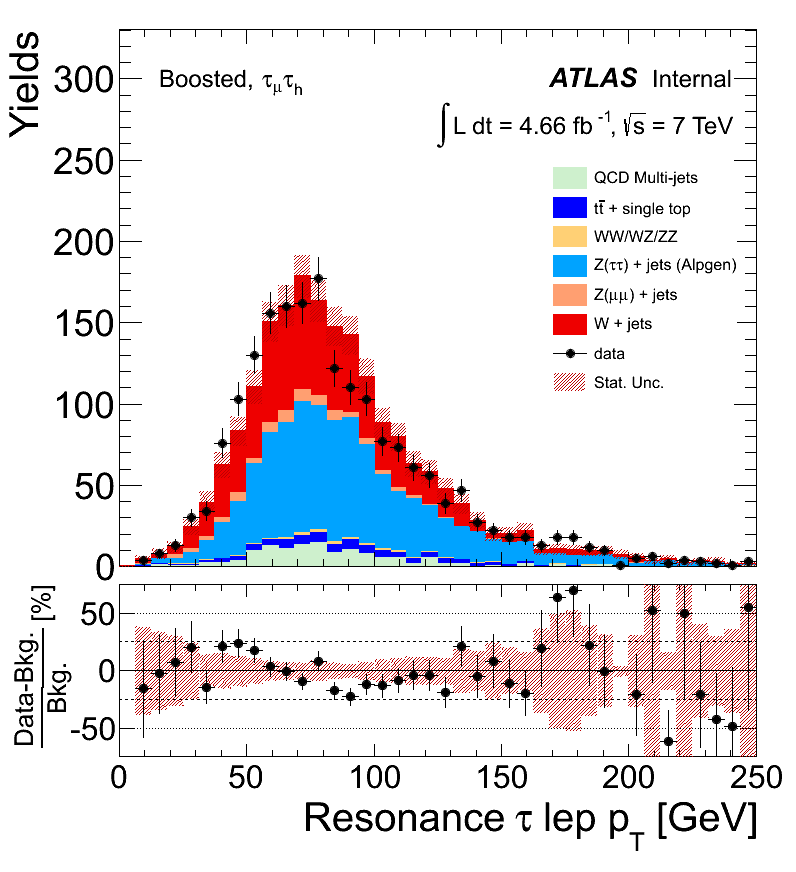
\includegraphics[width=\textwidth]{figures/lephad/mu_resonance_pt_tau_lep_boosted_sig.png}\\
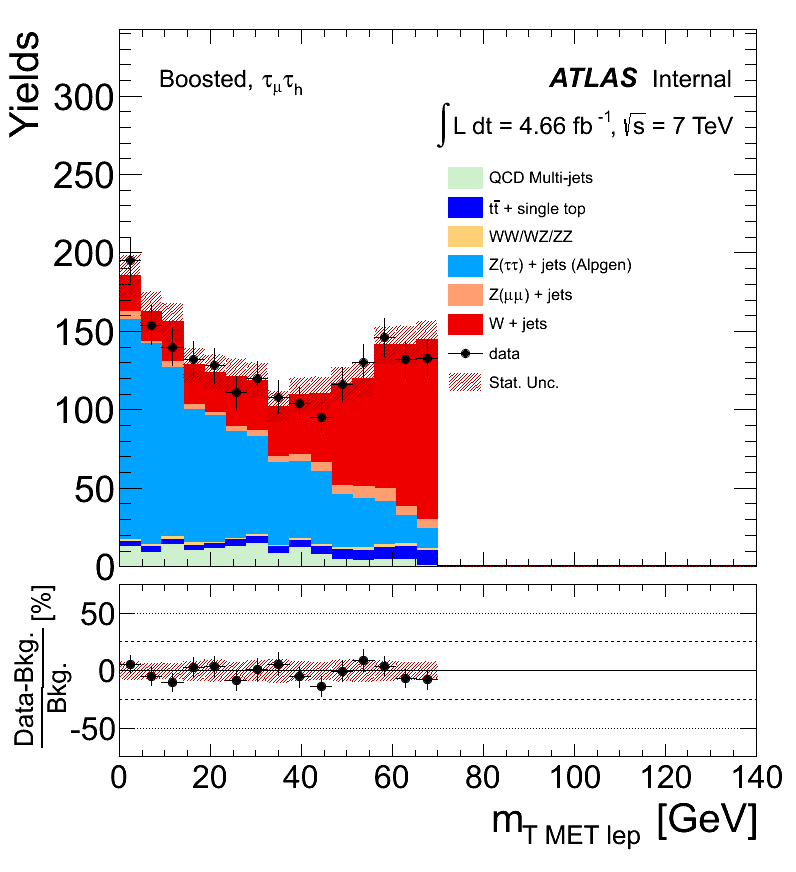
\includegraphics[width=\textwidth]{figures/lephad/mu_mass_transverse_met_lep_boosted_sig.png}
\column{0.3\textwidth}
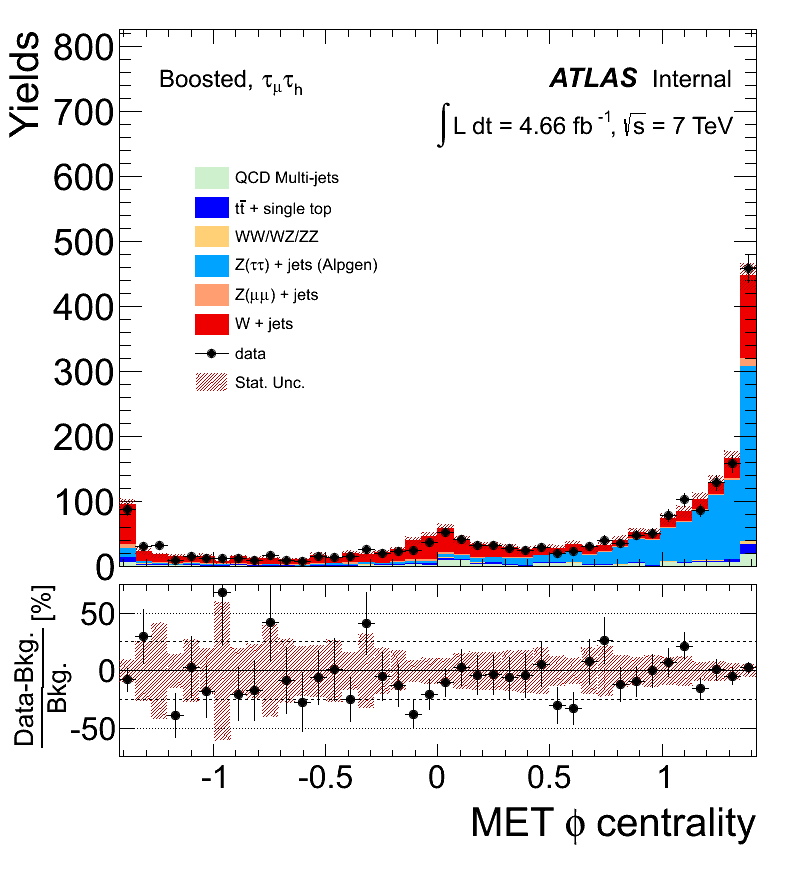
\includegraphics[width=\textwidth]{figures/lephad/mu_met_phi_centrality_boosted_sig.png}\\
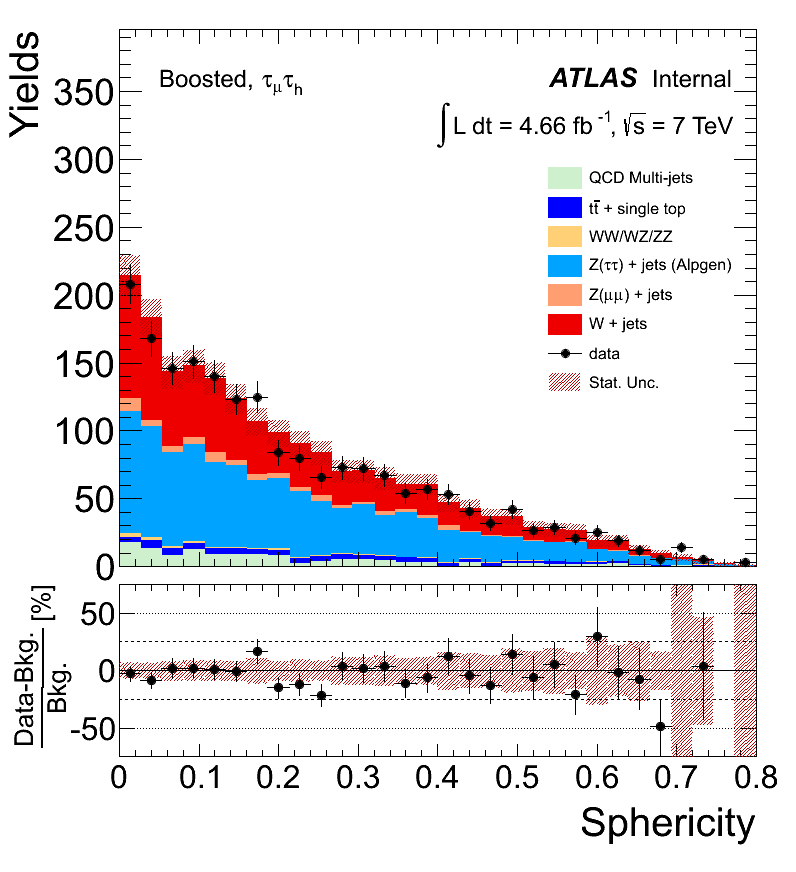
\includegraphics[width=\textwidth]{figures/lephad/mu_sphericity_boosted_sig.png}
\end{columns}


}

%%%
\frame{
\frametitle{Lephad Analysis - ggF(e) Discriminating Variables}

\begin{columns}
\column{0.3\textwidth}
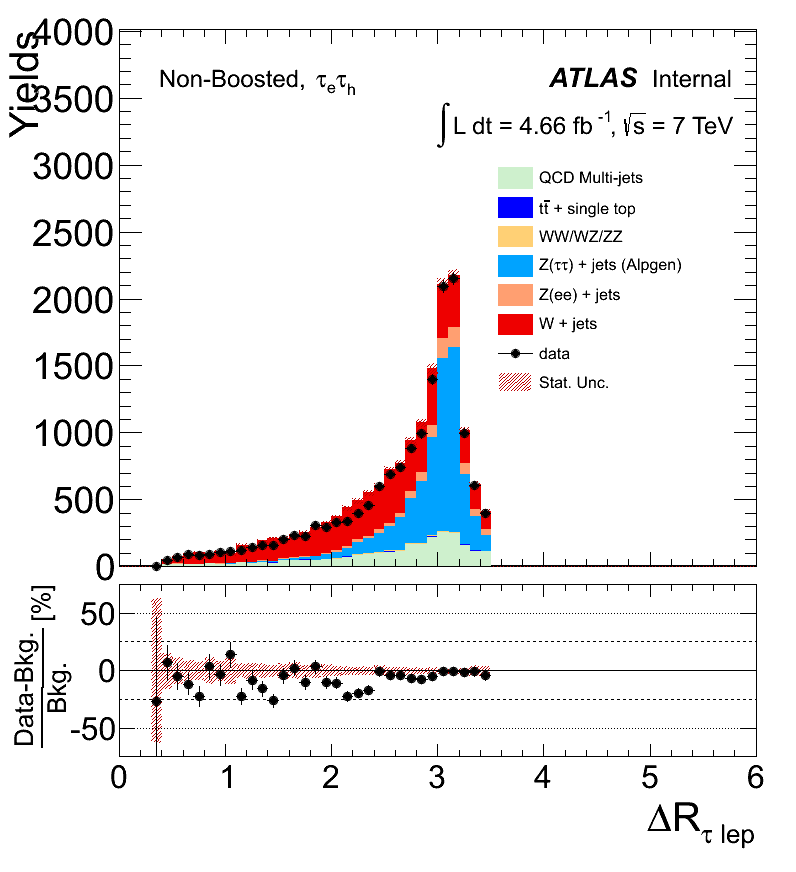
\includegraphics[width=\textwidth]{figures/lephad/e_dr_tau_lep_ggF_sig.png}\\
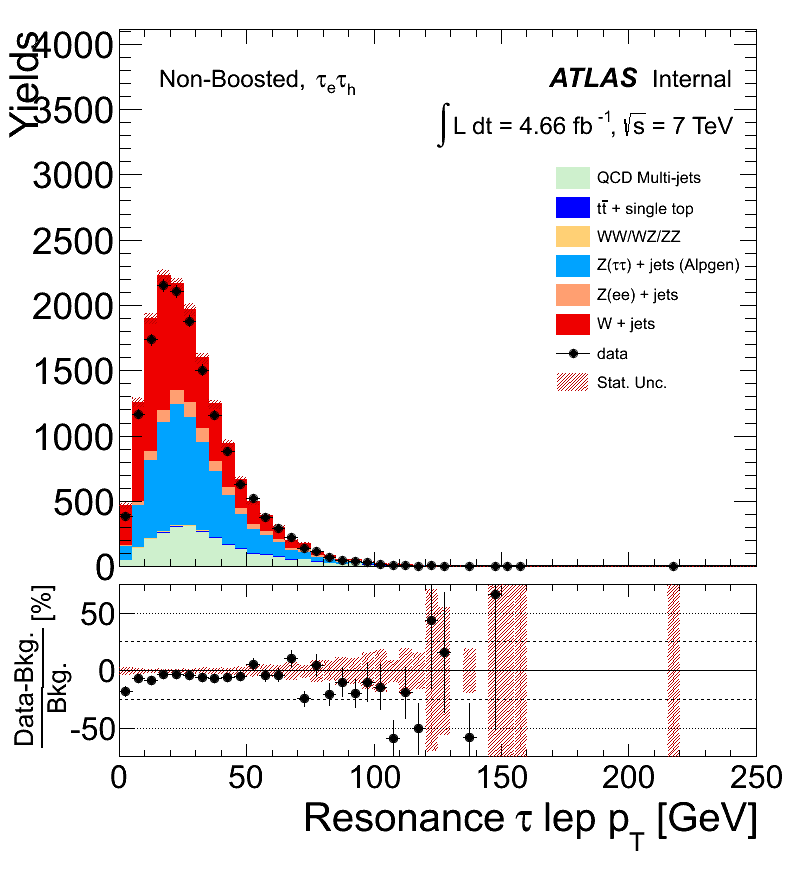
\includegraphics[width=\textwidth]{figures/lephad/e_resonance_pt_tau_lep_ggF_sig.png}
\column{0.3\textwidth}
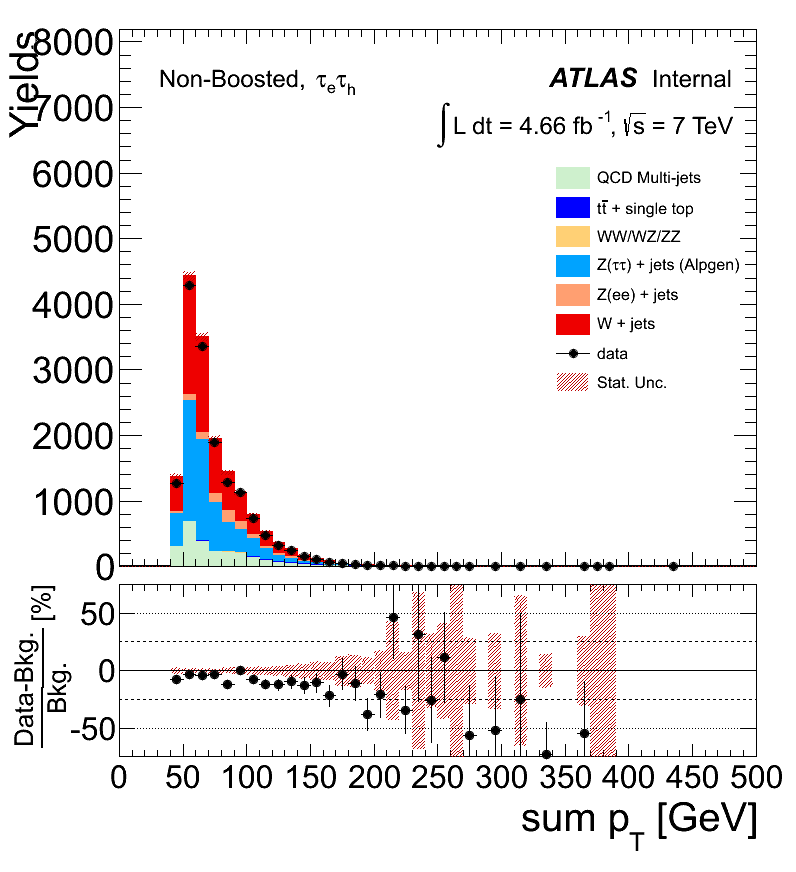
\includegraphics[width=\textwidth]{figures/lephad/e_sumPt_ggF_sig.png}\\
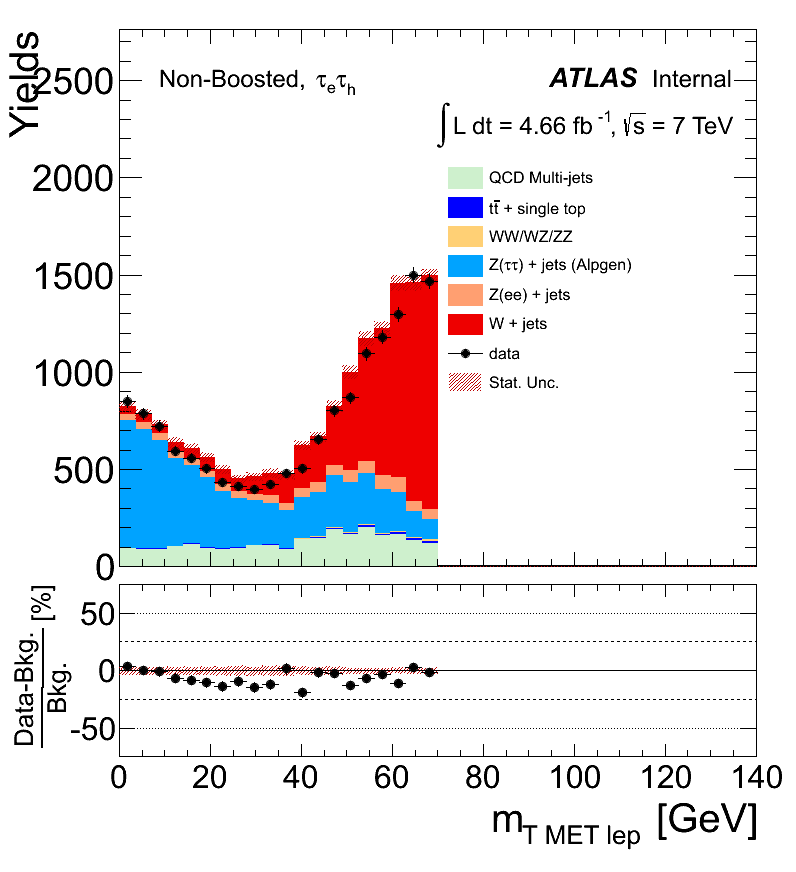
\includegraphics[width=\textwidth]{figures/lephad/e_mass_transverse_met_lep_ggF_sig.png}
\column{0.3\textwidth}
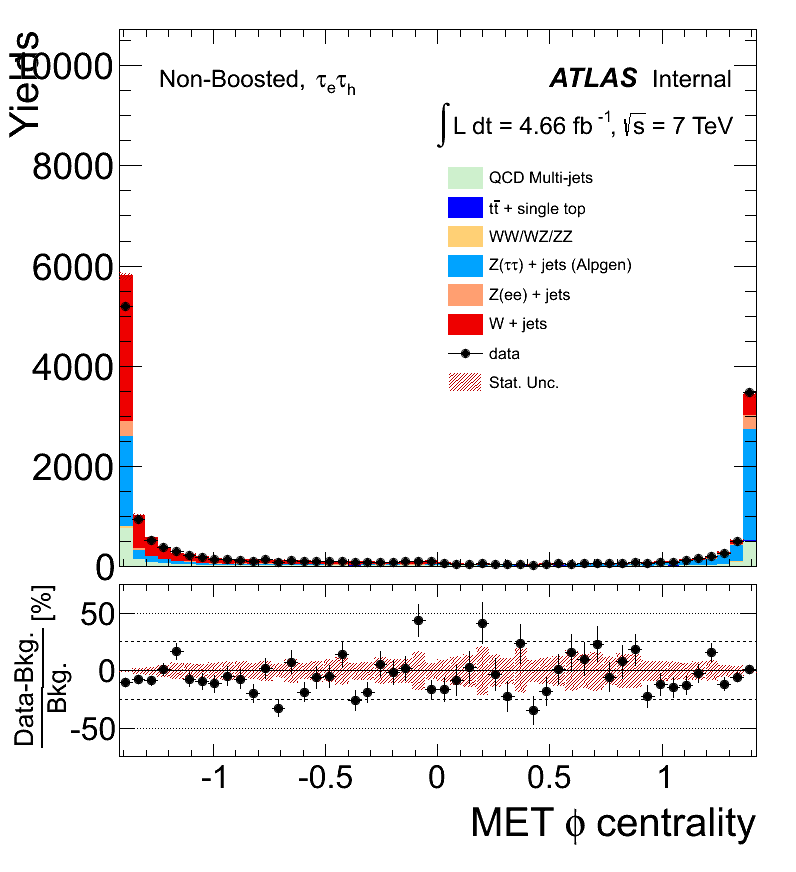
\includegraphics[width=\textwidth]{figures/lephad/e_met_phi_centrality_ggF_sig.png}\\

\end{columns}



}

%%%
\frame{
\frametitle{Lephad - Separating the Signal}

\begin{columns}
\column{0.3\textwidth}
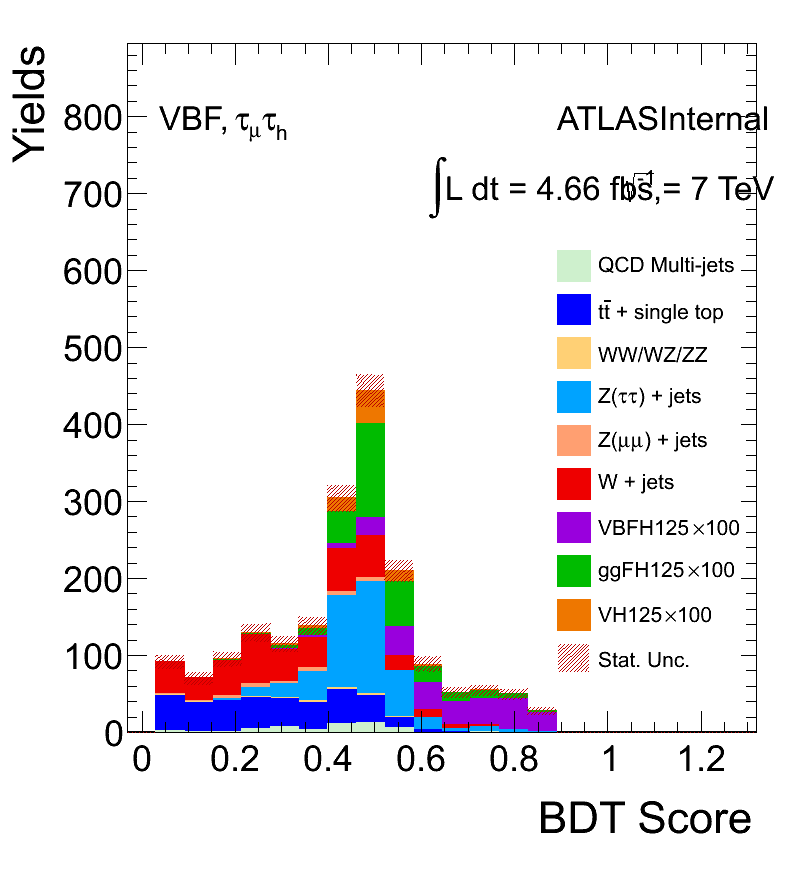
\includegraphics[width=\textwidth]{figures/lephad/mu_BDTScoreFull_VBF.png}\\
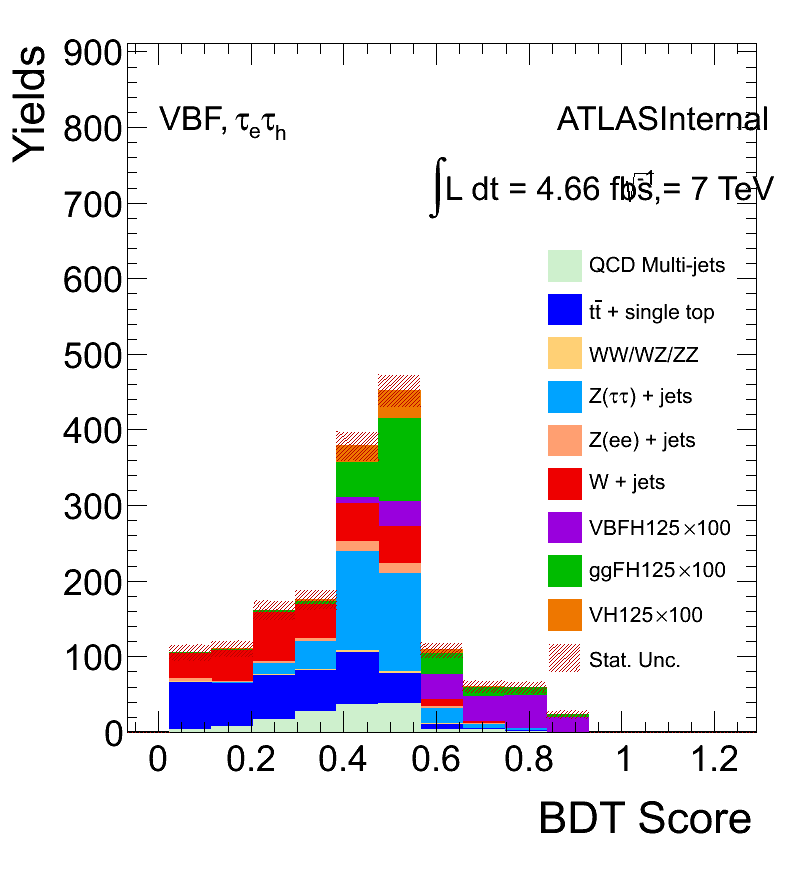
\includegraphics[width=\textwidth]{figures/lephad/e_BDTScoreFull_VBF.png}
\column{0.3\textwidth}
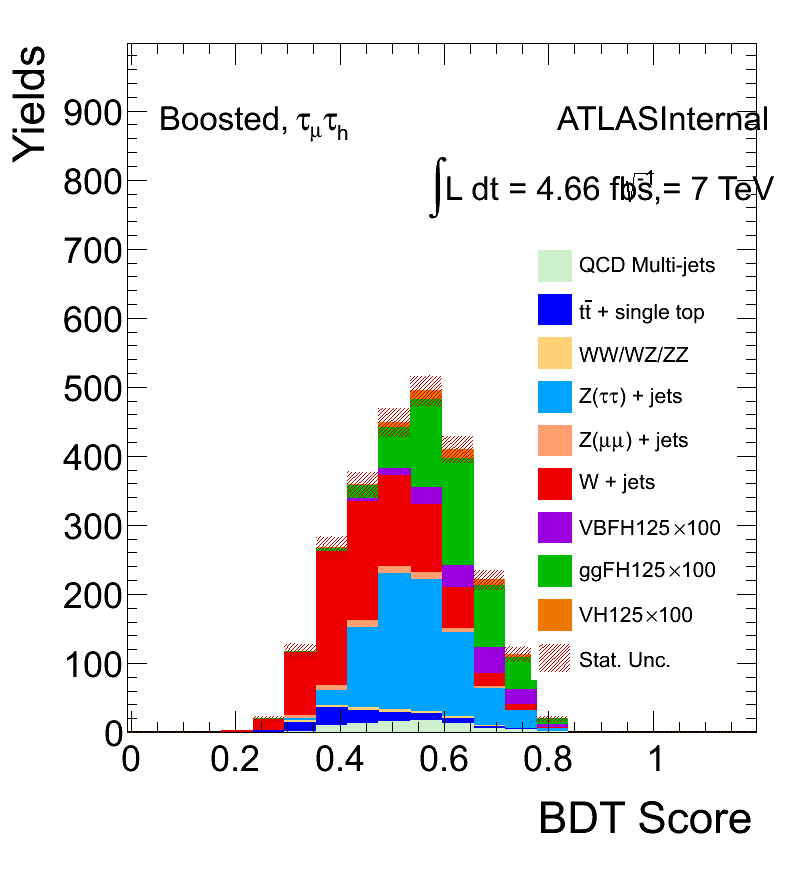
\includegraphics[width=\textwidth]{figures/lephad/mu_BDTScoreFull_boosted.png}\\
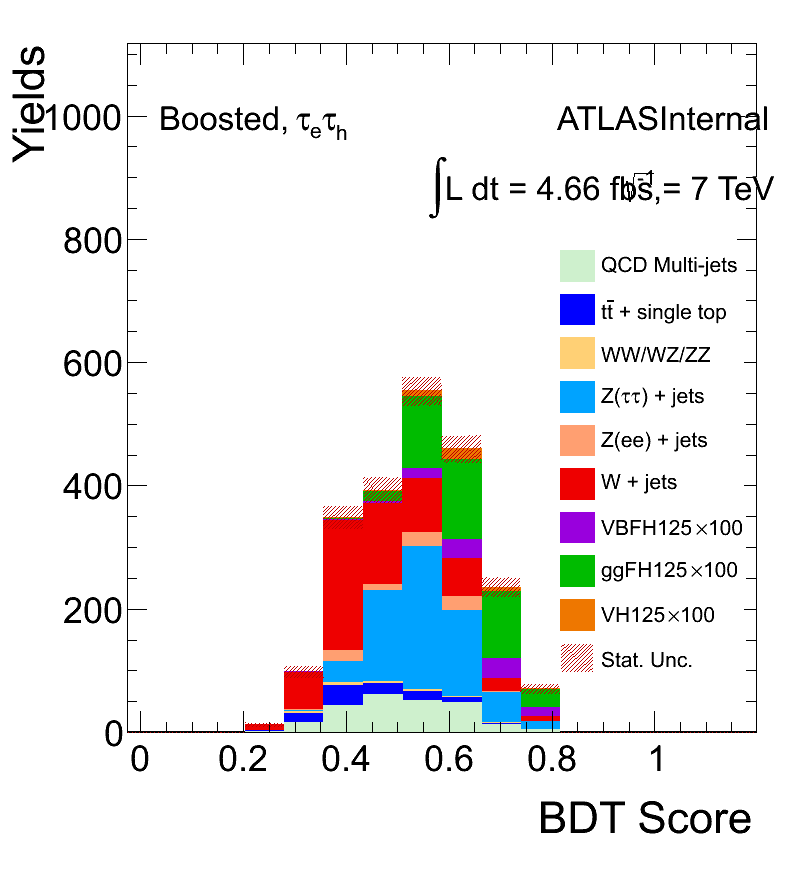
\includegraphics[width=\textwidth]{figures/lephad/e_BDTScoreFull_boosted.png}
\column{0.3\textwidth}
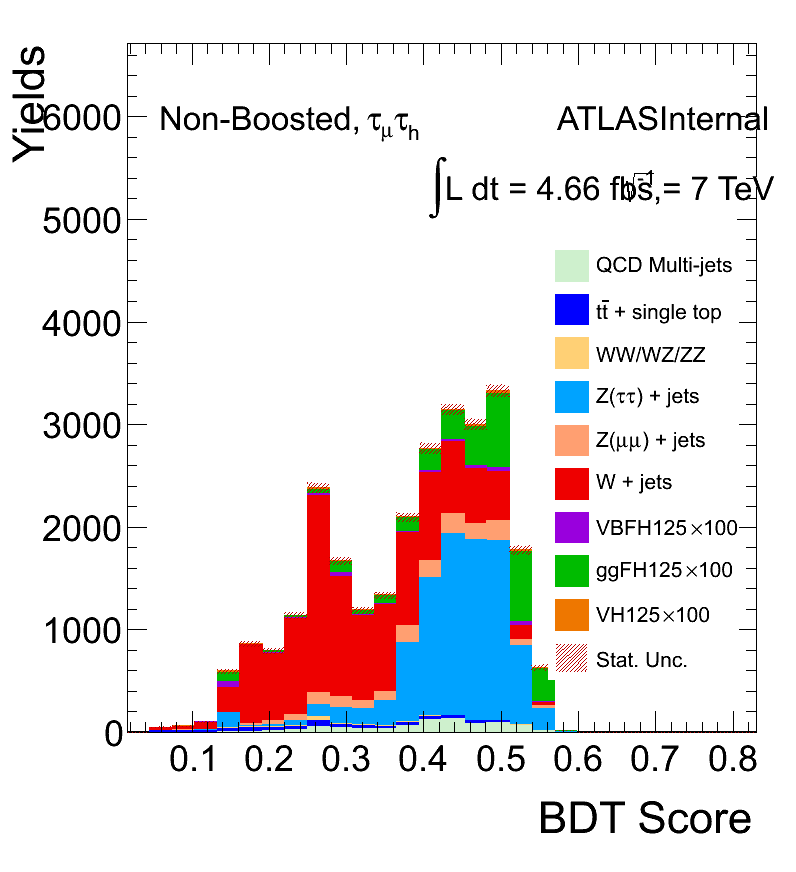
\includegraphics[width=\textwidth]{figures/lephad/mu_BDTScoreFull_ggF.png}\\
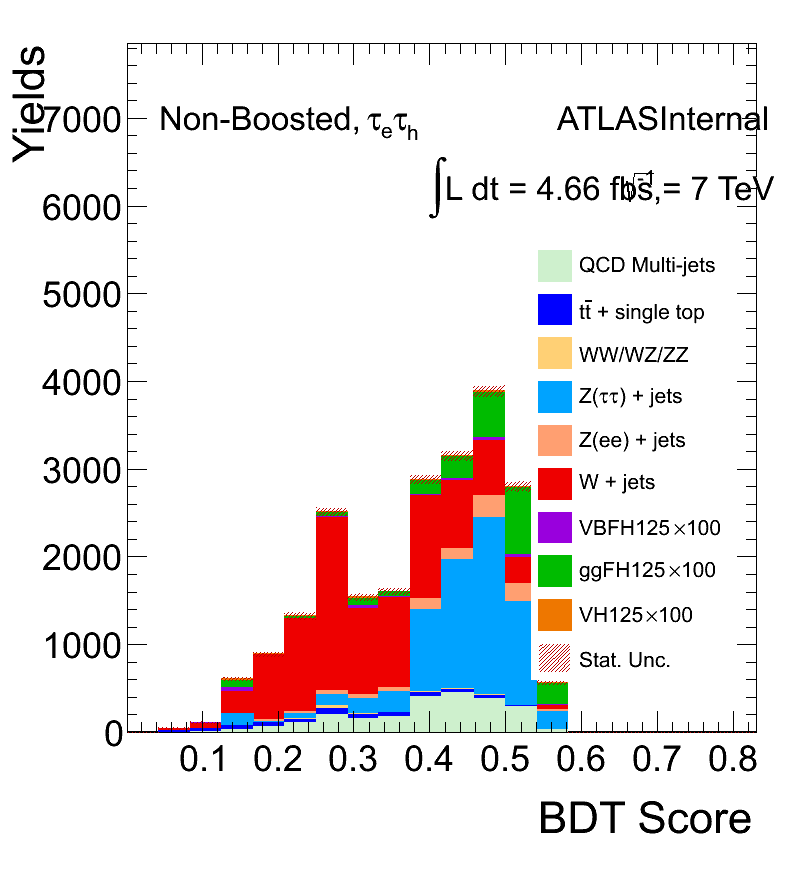
\includegraphics[width=\textwidth]{figures/lephad/e_BDTScoreFull_ggF.png}
\end{columns}

}

%%%
\frame{
\frametitle{Lephad Mass Sideband Controls}

\begin{columns}
\column{0.3\textwidth}
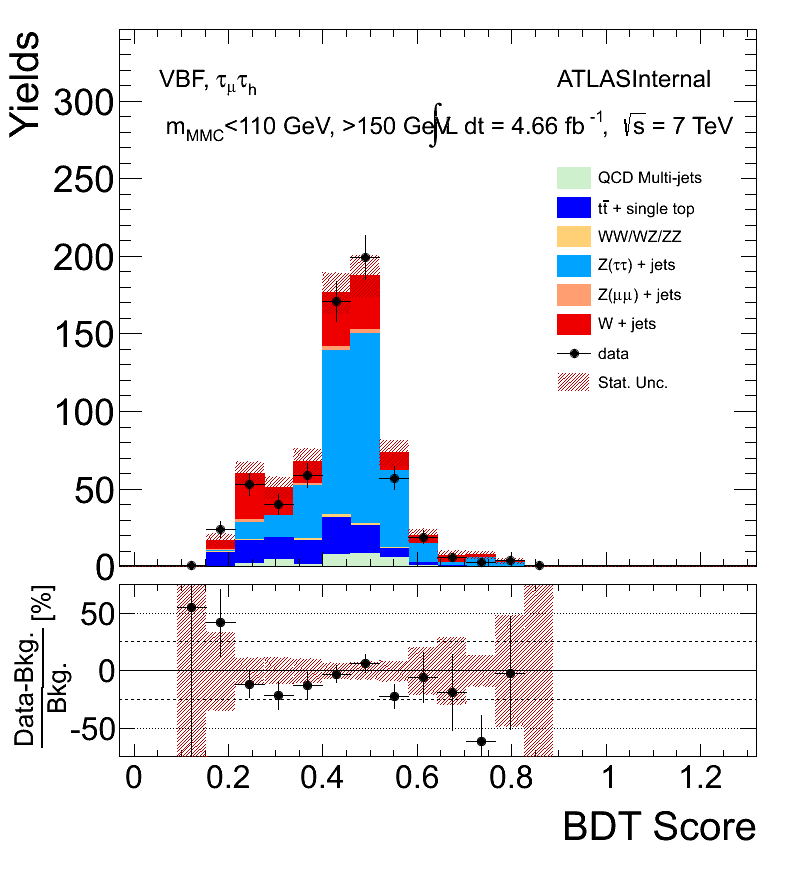
\includegraphics[width=\textwidth]{figures/lephad/mu_BDTScoreFull_VBF_controlS.png}\\
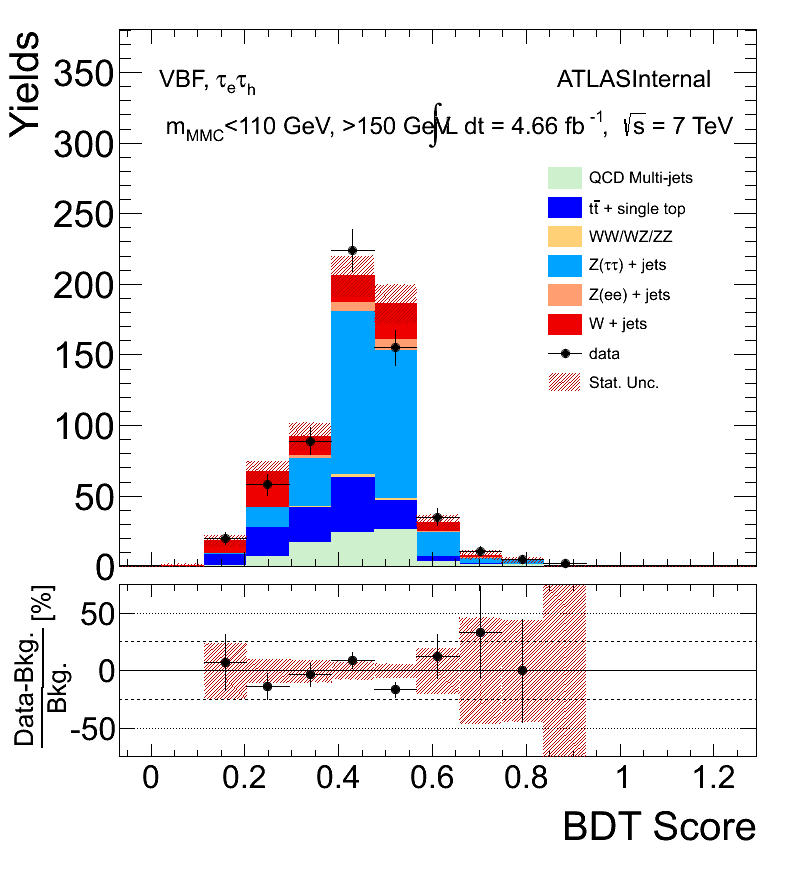
\includegraphics[width=\textwidth]{figures/lephad/e_BDTScoreFull_VBF_controlS.png}
\column{0.3\textwidth}
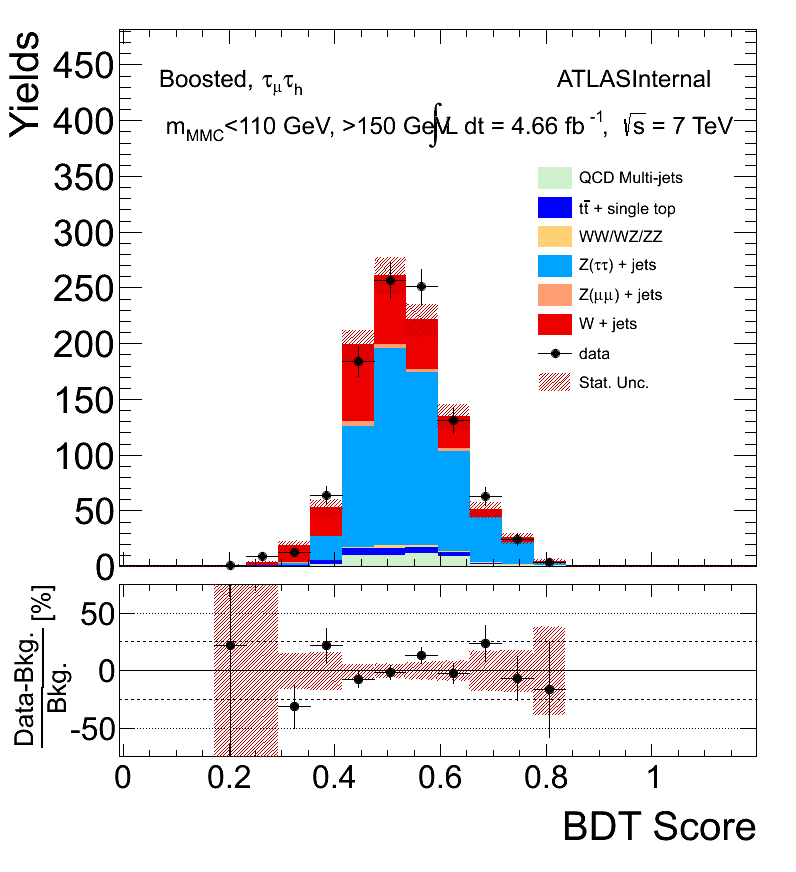
\includegraphics[width=\textwidth]{figures/lephad/mu_BDTScoreFull_boosted_controlS.png}\\
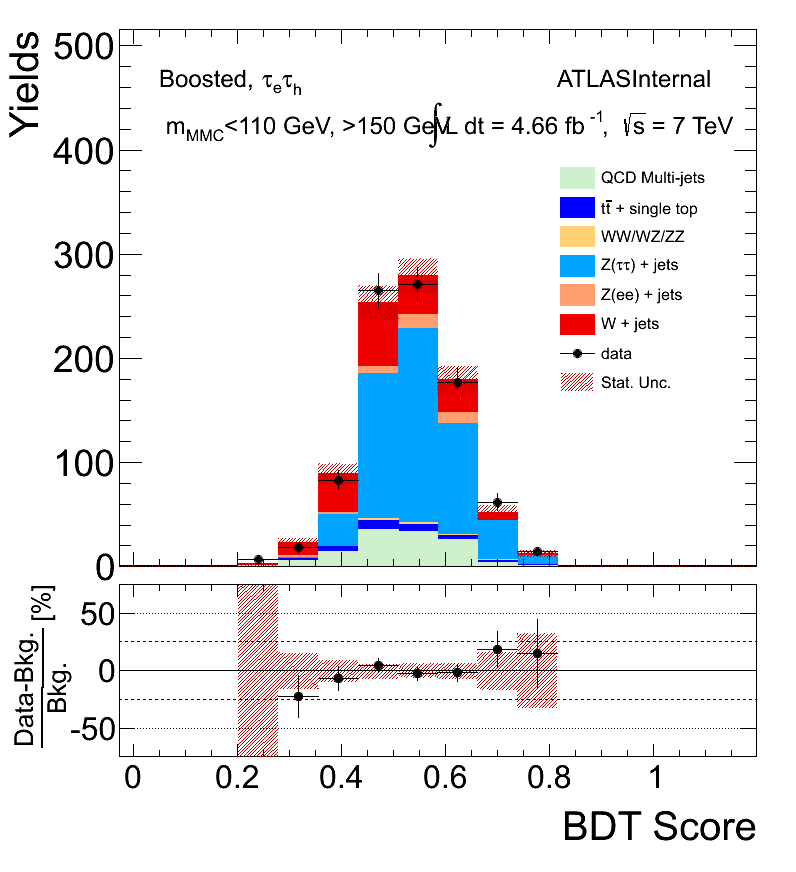
\includegraphics[width=\textwidth]{figures/lephad/e_BDTScoreFull_boosted_controlS.png}
\column{0.3\textwidth}
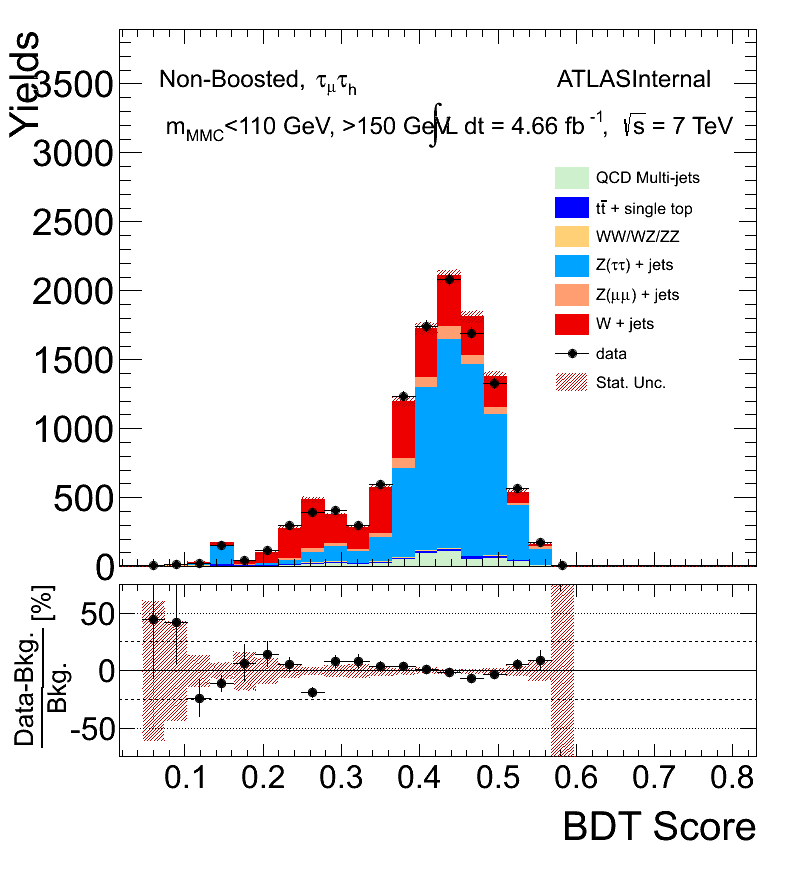
\includegraphics[width=\textwidth]{figures/lephad/mu_BDTScoreFull_ggF_controlS.png}\\
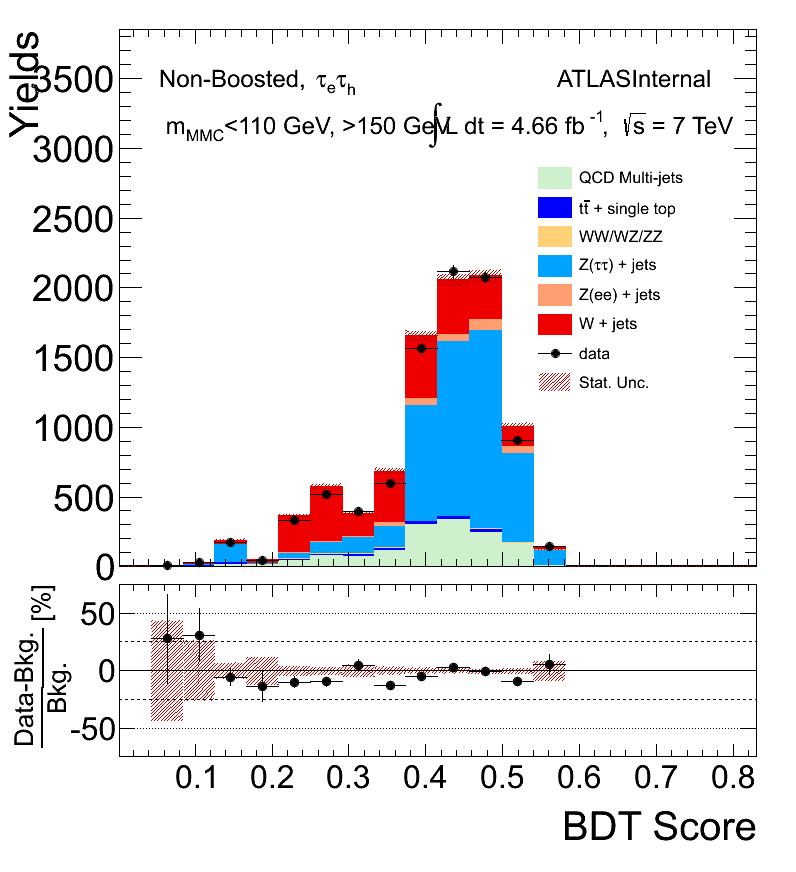
\includegraphics[width=\textwidth]{figures/lephad/e_BDTScoreFull_ggF_controlS.png}
\end{columns}


}

%%%
\frame{
\frametitle{Lephad W Controls}

\begin{columns}
\column{0.3\textwidth}
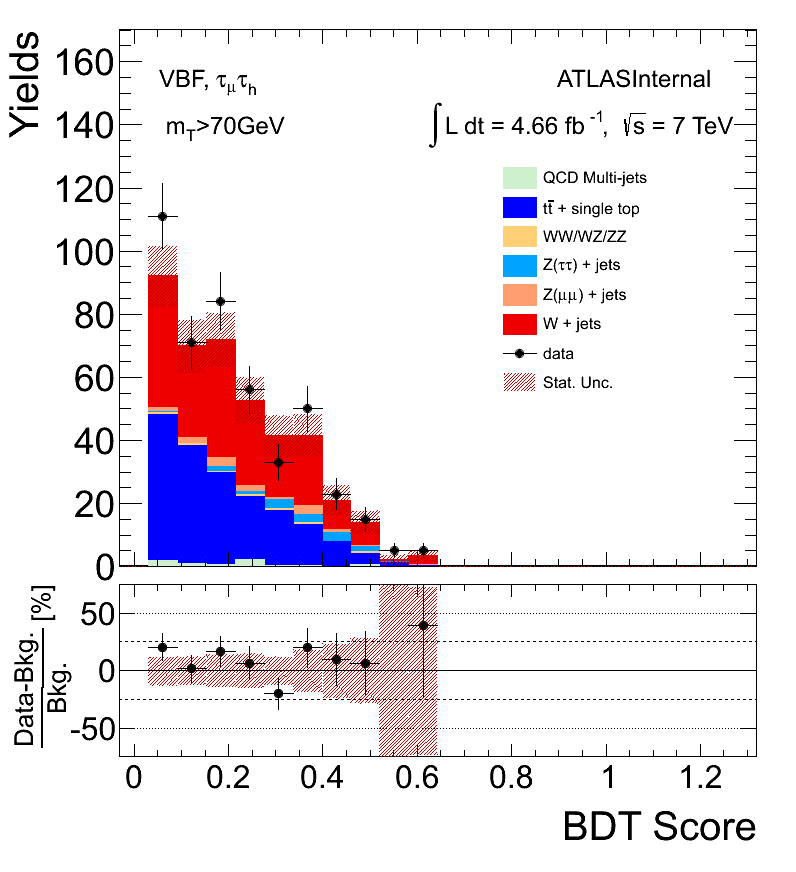
\includegraphics[width=\textwidth]{figures/lephad/mu_BDTScoreFull_VBF_controlW.png}\\
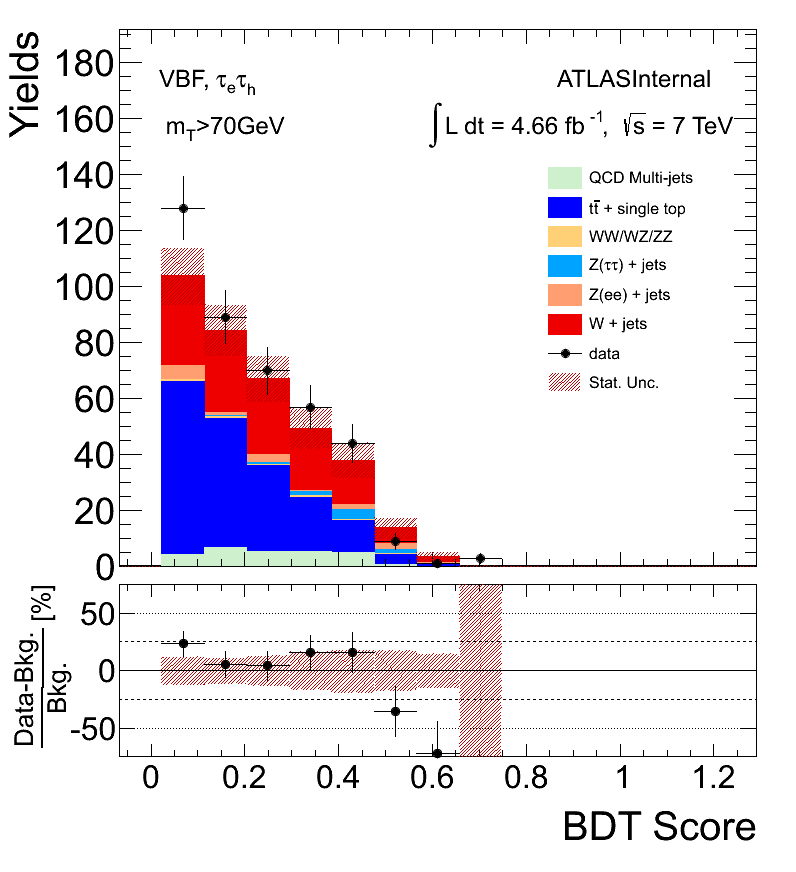
\includegraphics[width=\textwidth]{figures/lephad/e_BDTScoreFull_VBF_controlW.png}
\column{0.3\textwidth}
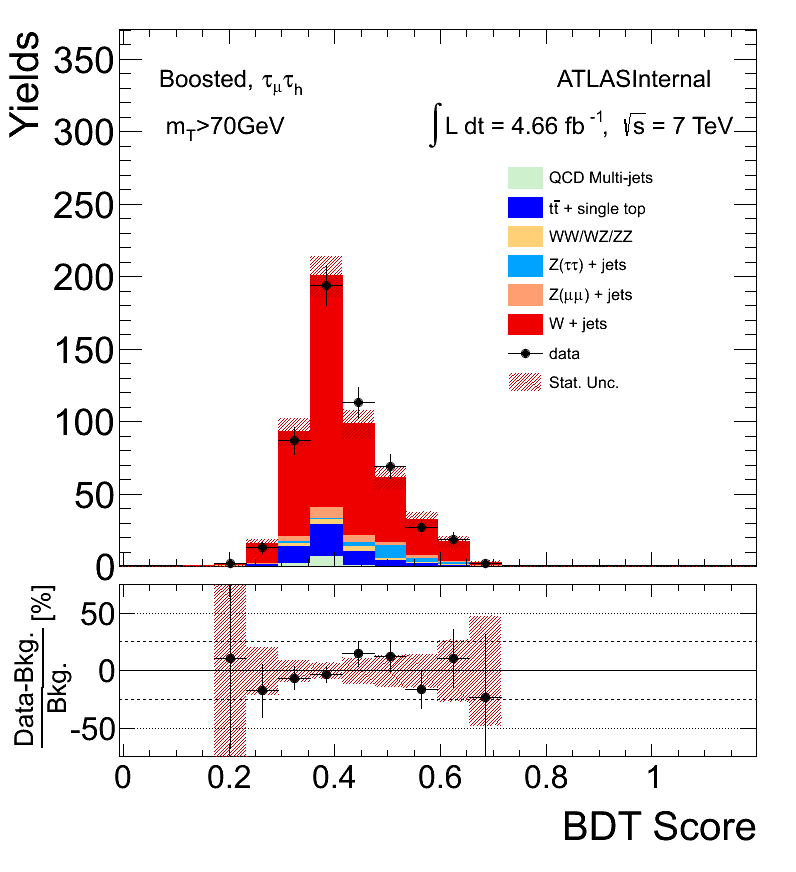
\includegraphics[width=\textwidth]{figures/lephad/mu_BDTScoreFull_boosted_controlW.png}\\
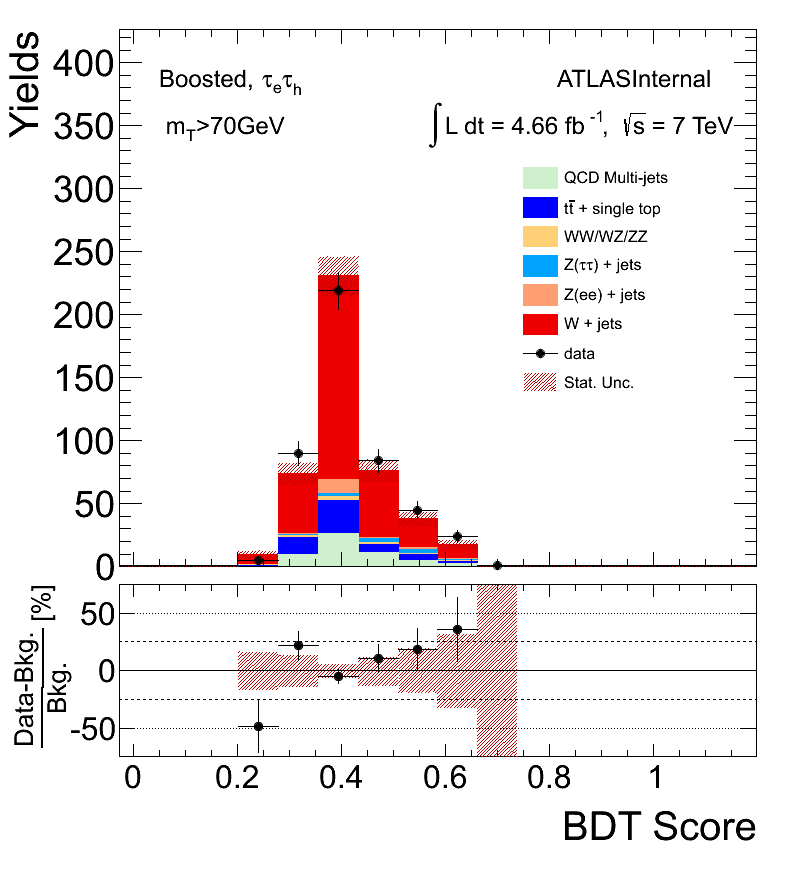
\includegraphics[width=\textwidth]{figures/lephad/e_BDTScoreFull_boosted_controlW.png}
\column{0.3\textwidth}
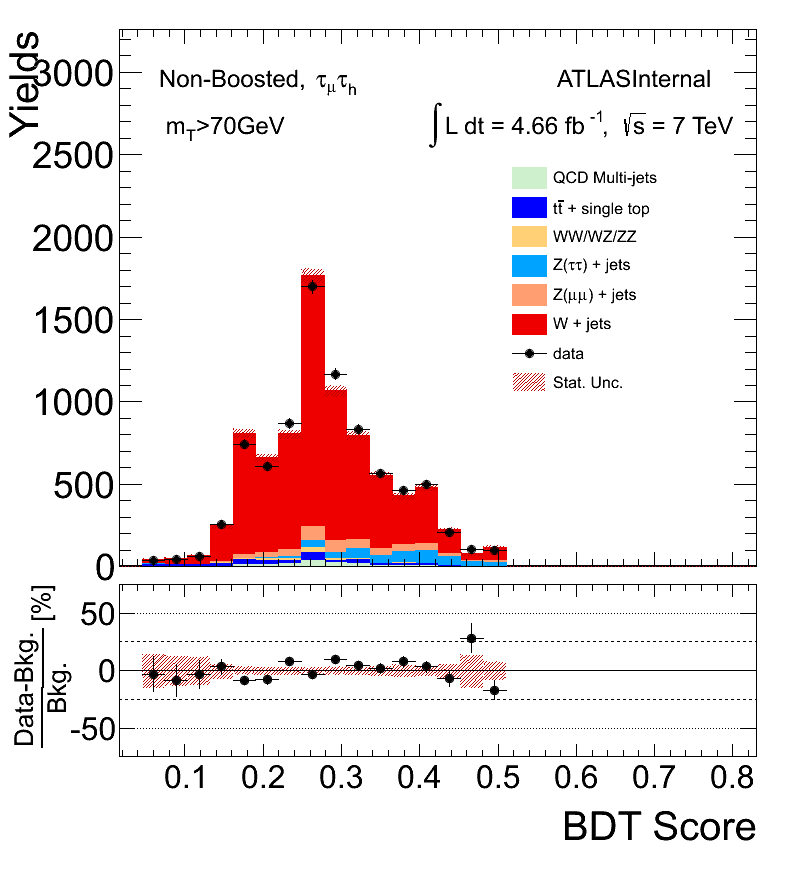
\includegraphics[width=\textwidth]{figures/lephad/mu_BDTScoreFull_ggF_controlW.png}\\
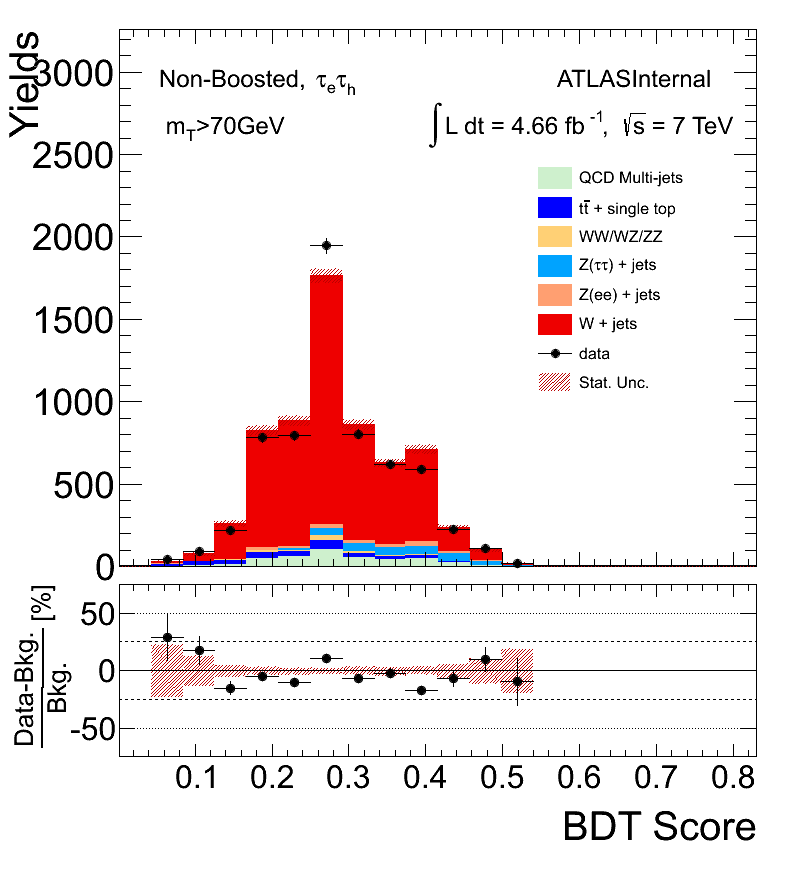
\includegraphics[width=\textwidth]{figures/lephad/e_BDTScoreFull_ggF_controlW.png}
\end{columns}
}

%%%
\frame{
\frametitle{Lephad Z Controls}

\begin{columns}
\column{0.3\textwidth}
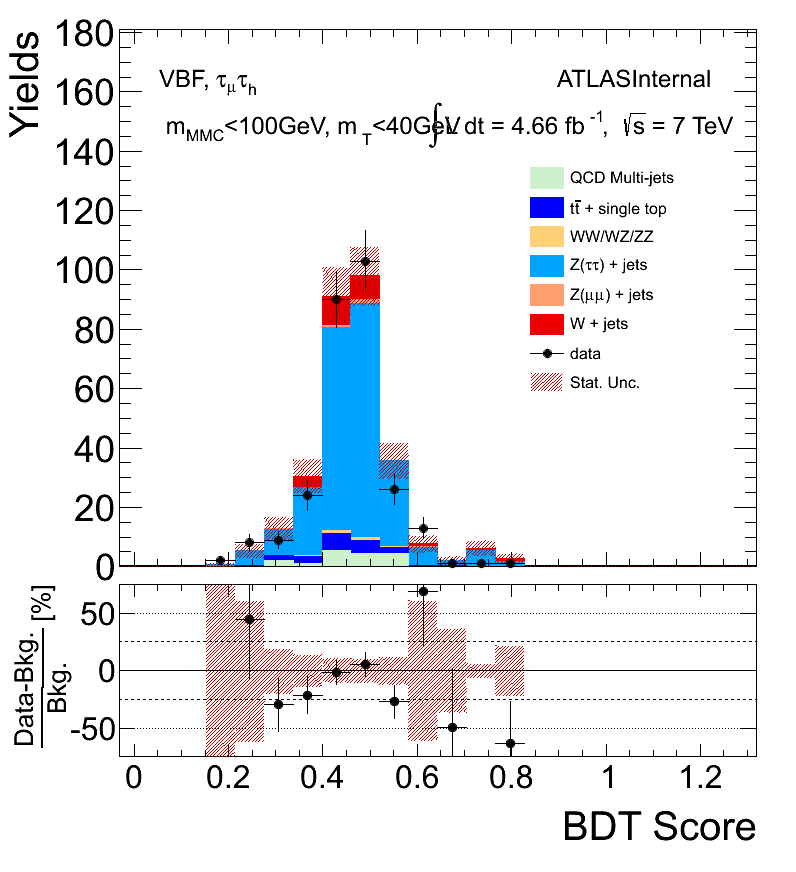
\includegraphics[width=\textwidth]{figures/lephad/mu_BDTScoreFull_VBF_controlZ.png}\\
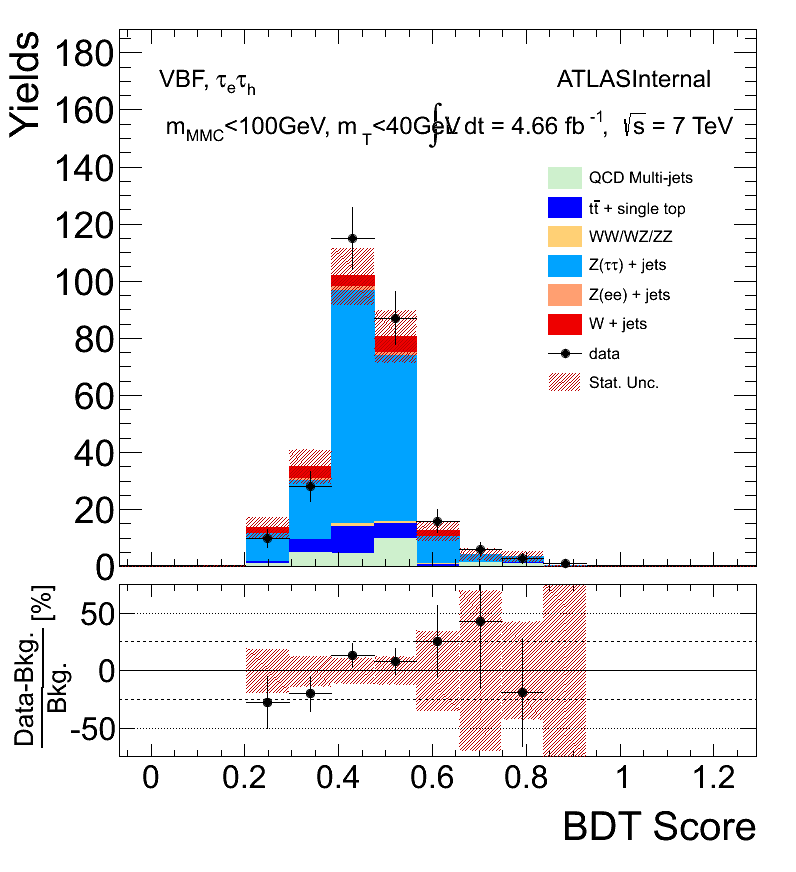
\includegraphics[width=\textwidth]{figures/lephad/e_BDTScoreFull_VBF_controlZ.png}
\column{0.3\textwidth}
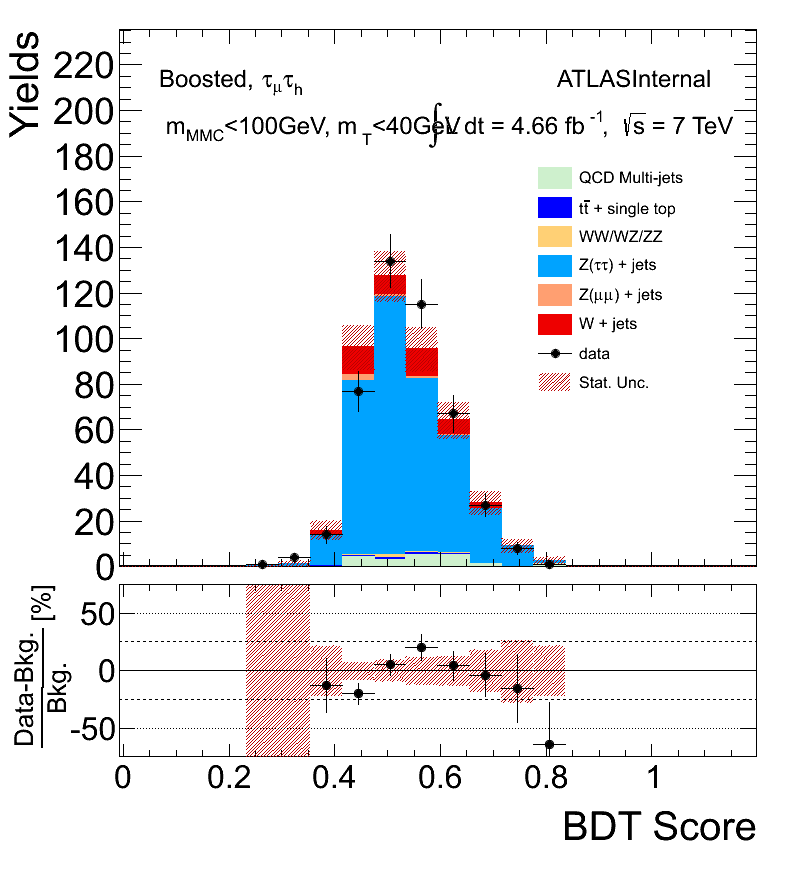
\includegraphics[width=\textwidth]{figures/lephad/mu_BDTScoreFull_boosted_controlZ.png}\\
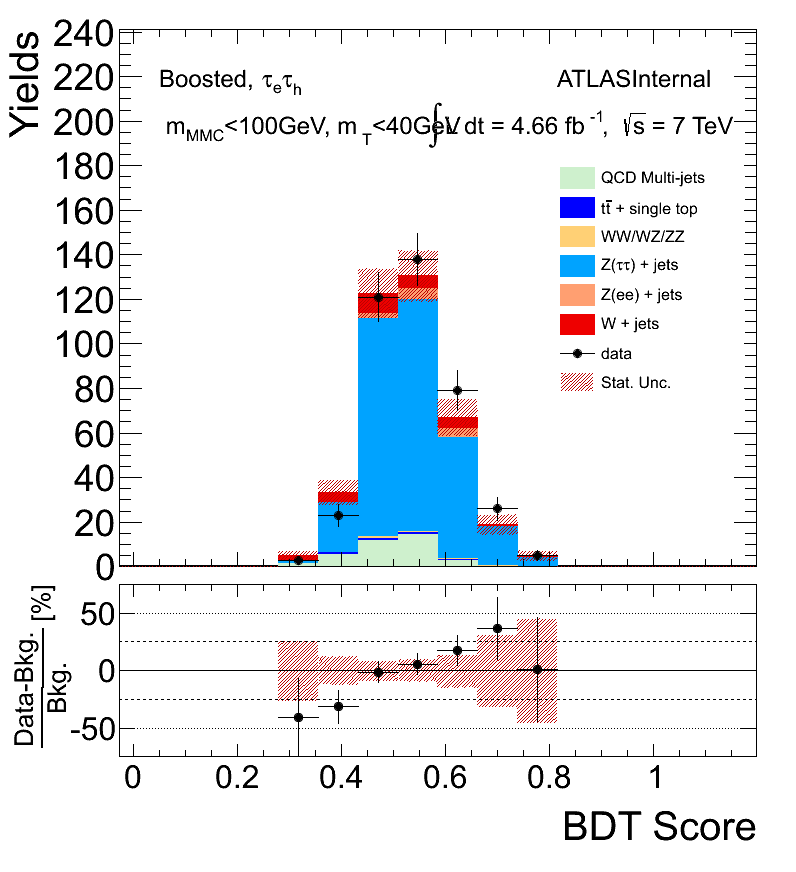
\includegraphics[width=\textwidth]{figures/lephad/e_BDTScoreFull_boosted_controlZ.png}
\column{0.3\textwidth}
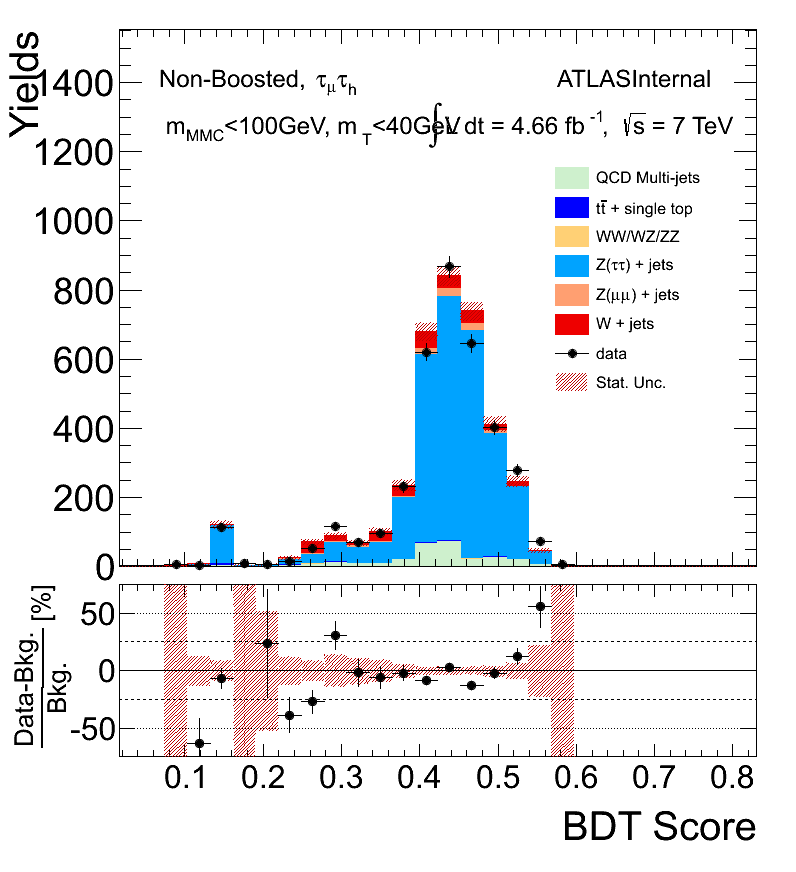
\includegraphics[width=\textwidth]{figures/lephad/mu_BDTScoreFull_ggF_controlZ.png}\\
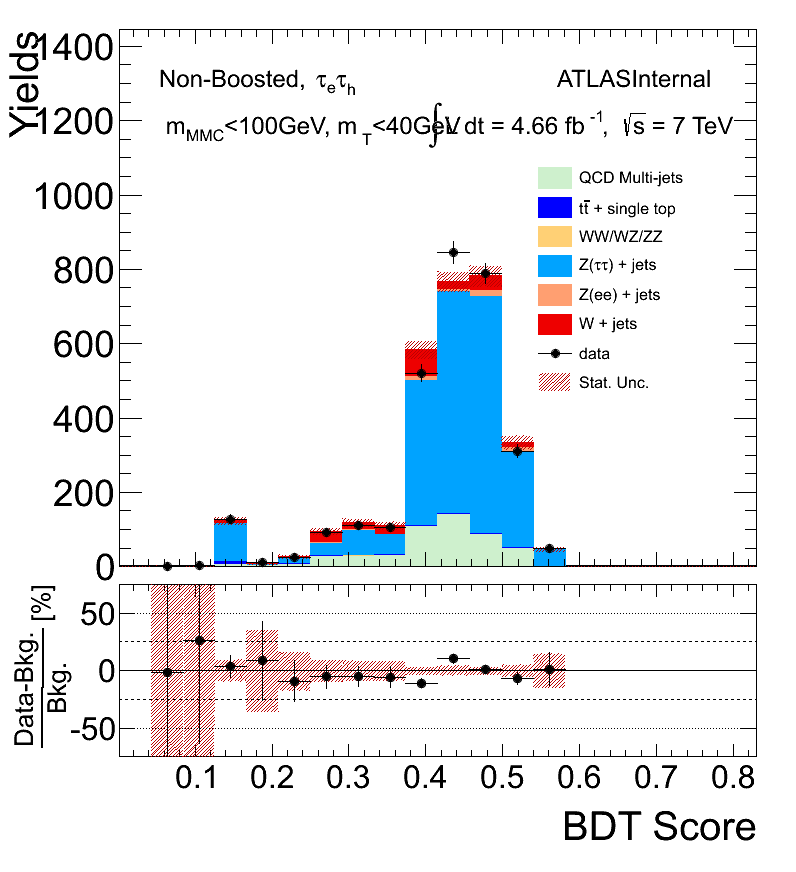
\includegraphics[width=\textwidth]{figures/lephad/e_BDTScoreFull_ggF_controlZ.png}
\end{columns}


}

%%%
\frame{
\frametitle{Lephad Expected Limits}

\begin{columns}
\column{0.45\textwidth}
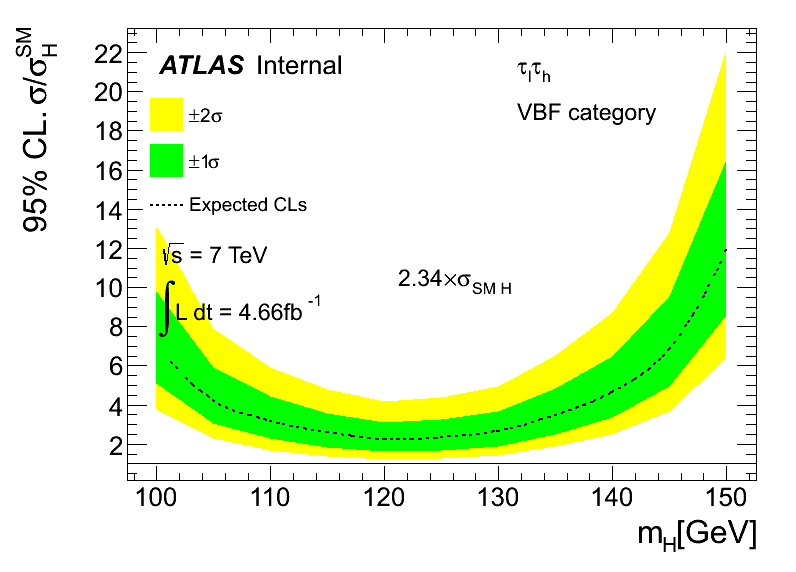
\includegraphics[width=\textwidth]{figures/lephad/LimitBand_VBFLH.png}\\
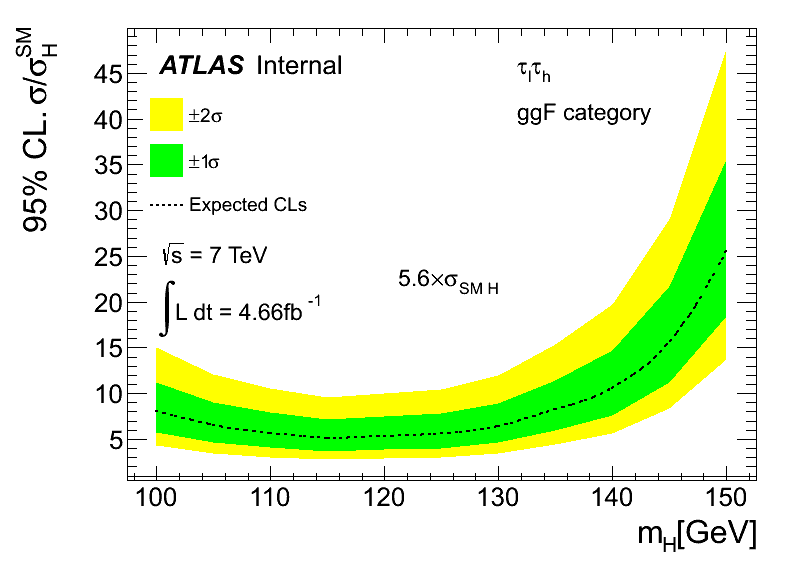
\includegraphics[width=\textwidth]{figures/lephad/LimitBand_ggFLH.png}
\column{0.45\textwidth}
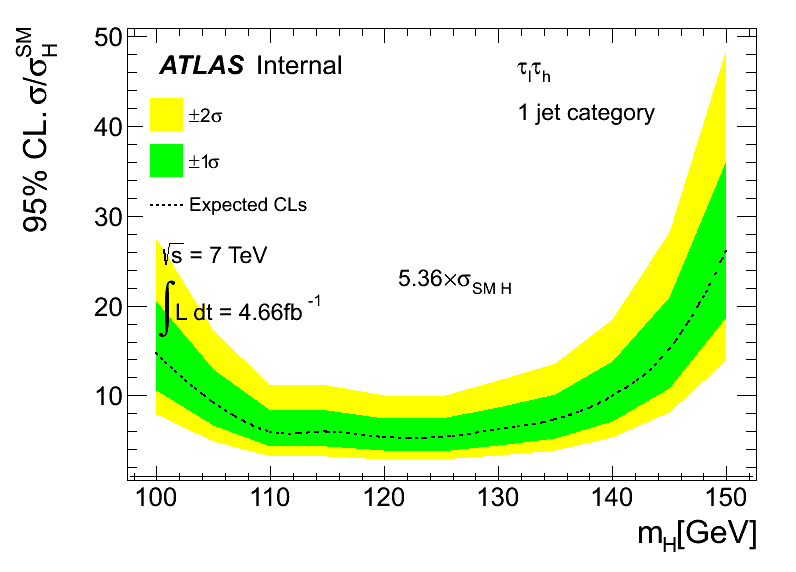
\includegraphics[width=\textwidth]{figures/lephad/LimitBand_boostedLH.png}\\
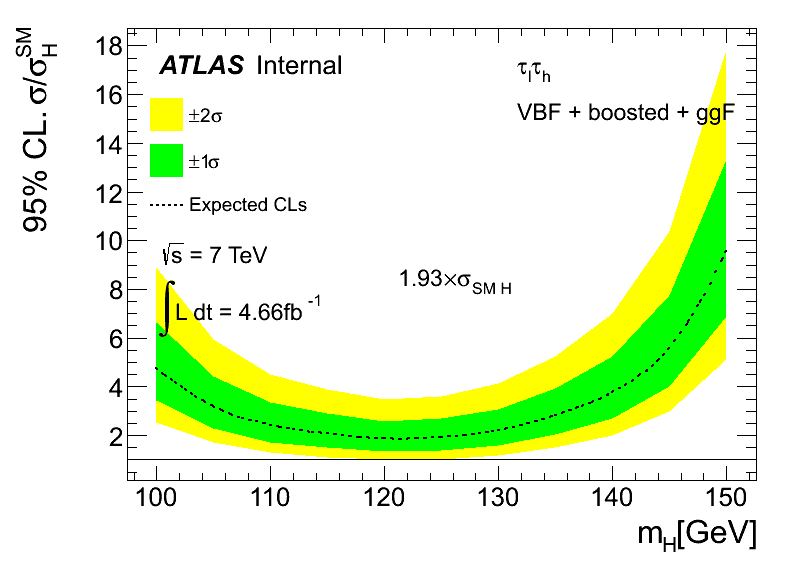
\includegraphics[width=\textwidth]{figures/lephad/LimitBand_combined.png}
\end{columns}


}


%%%
%%%
\frame{
\frametitle{Hadhad Analysis Intro}

\begin{itemize}

\item Dominant background contributions are different: QCD multi-jets is far more important, EWK backgrounds are almost negligible.

\item Requires a different set of variable lists - though many
  variables are also common with lephad. QCD multi-jets suppression
  variables gain importance, EWK suppression is less important.

\item Not as many available control regions in this channel.

\item Using TauID BDT score as a variable in non-VBF categories to
  suppress QCD. Requires special uncertainty treatment. \href{https://indico.cern.ch/getFile.py/access?contribId=3&resId=0&materialId=slides&confId=205496}{Presented} to TauWG recently.

\item Note: error bands for hadhad validation plots include full
  shape-varying systematics.

\end{itemize}

}

%%%
%%%
\frame{
\frametitle{Hadhad Analysis - TauID BDT Uncertainty}

\begin{center}
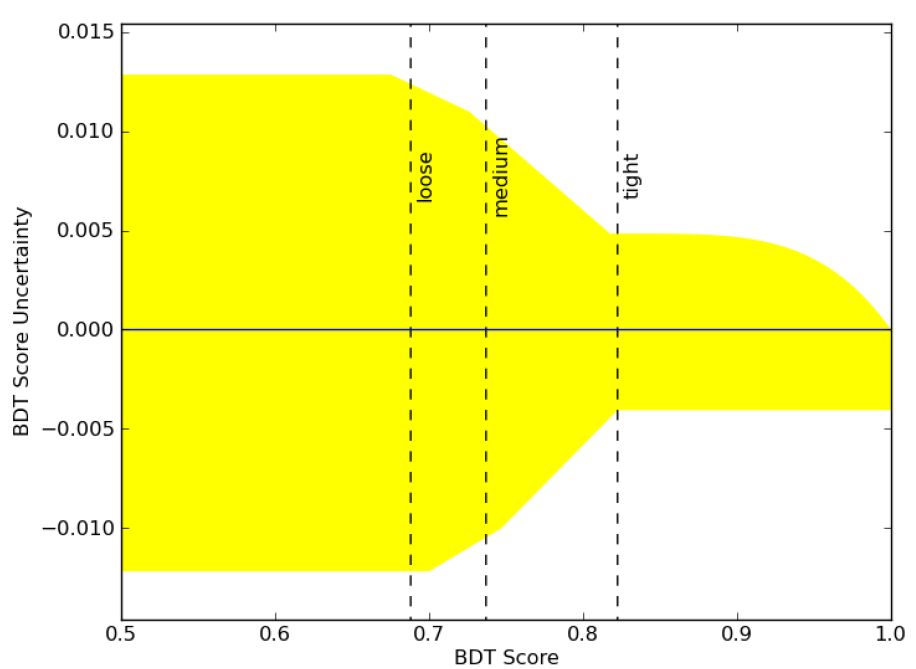
\includegraphics[width=0.85\textwidth]{figures/hadhad/TauID-BDT-uncertainty.png}
\end{center}

}

%%%
\frame{
\frametitle{Hadhad Analysis - VBF  Discriminating Variables}

% First 6 Boosted distinguishing variables (highest ranked).

\begin{columns}
\column{0.3\textwidth}
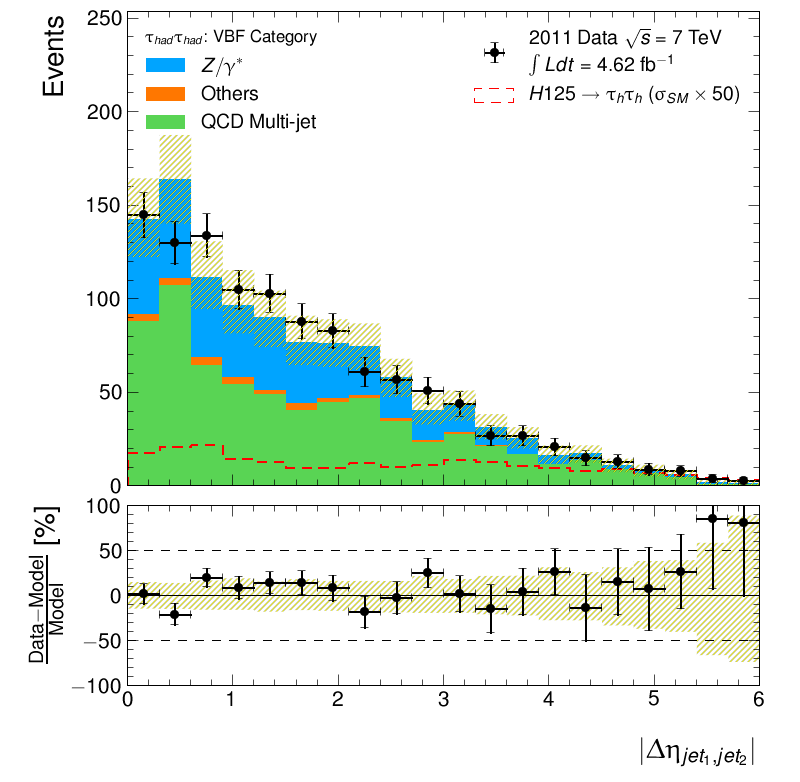
\includegraphics[width=\textwidth]{figures/hadhad/var_vbf_deta_jets.png}\\
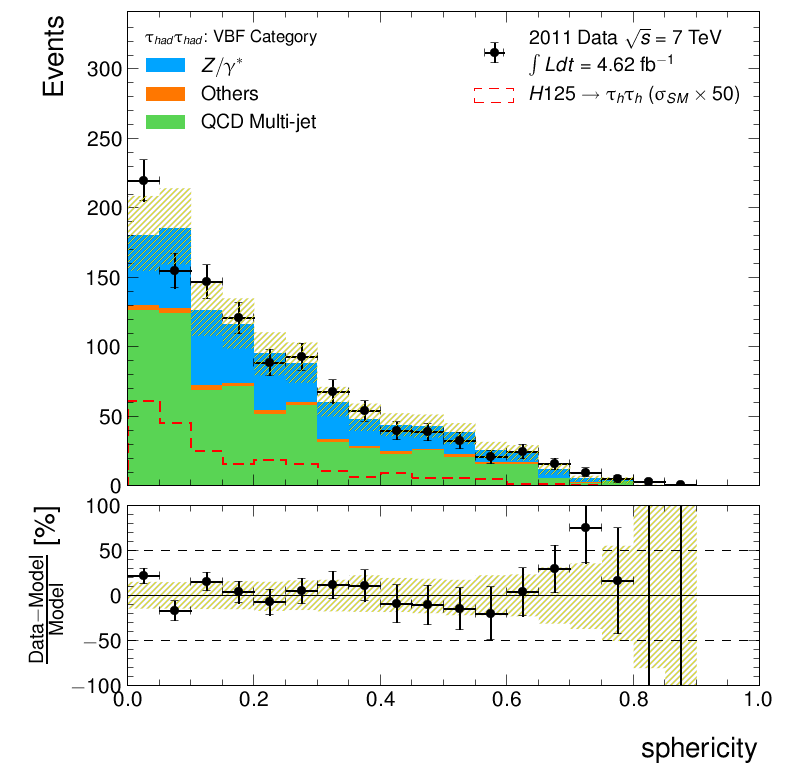
\includegraphics[width=\textwidth]{figures/hadhad/var_vbf_sphericity.png}
\column{0.3\textwidth}
\includegraphics[width=\textwidth]{figures/hadhad/var_vbf_eta_product_jets.png}\\
\includegraphics[width=\textwidth]{figures/hadhad/var_vbf_tau1_centrality.png}
\column{0.3\textwidth}
\includegraphics[width=\textwidth]{figures/hadhad/var_vbf_m_jet1_jet2.png}\\
\includegraphics[width=\textwidth]{figures/hadhad/var_vbf_tau2_centrality.png}
\end{columns}


}

%%%
\frame{
\frametitle{Hadhad Analysis - Boosted Discriminating Variables}

%First 6 Boosted distinguishing variables (highest ranked).

\begin{columns}
\column{0.3\textwidth}
\includegraphics[width=\textwidth]{figures/hadhad/var_boosted_sphericity.png}\\
\includegraphics[width=\textwidth]{figures/hadhad/var_boosted_tau2_bdtjetscore.png}
\column{0.3\textwidth}
\includegraphics[width=\textwidth]{figures/hadhad/var_boosted_dr_tau1_tau2.png}\\
\includegraphics[width=\textwidth]{figures/hadhad/var_boosted_tau1_x.png}
\column{0.3\textwidth}
\includegraphics[width=\textwidth]{figures/hadhad/var_boosted_tau1_bdtjetscore.png}\\
\includegraphics[width=\textwidth]{figures/hadhad/var_boosted_tau2_x.png}
\end{columns}

}

%%%
\frame{
\frametitle{Hadhad Analysis - ggF Discriminating Variables}

%All 6 ggF distinguishing variables.

\begin{columns}
\column{0.3\textwidth}
\includegraphics[width=\textwidth]{figures/hadhad/var_ggf_dr_tau1_tau2.png}\\
\includegraphics[width=\textwidth]{figures/hadhad/var_ggf_tau1_x.png}
\column{0.3\textwidth}
\includegraphics[width=\textwidth]{figures/hadhad/var_ggf_tau1_bdtjetscore.png}\\
\includegraphics[width=\textwidth]{figures/hadhad/var_ggf_tau2_x.png}
\column{0.3\textwidth}
\includegraphics[width=\textwidth]{figures/hadhad/var_ggf_tau2_bdtjetscore.png}\\
\includegraphics[width=\textwidth]{figures/hadhad/var_ggf_met_centrality.png}
\end{columns}


}

%%%
\frame{
\frametitle{hadhad Mass Sideband Controls}

All 3 sideband BDT control distributions. 

}


%%%
%%%
\frame{
\frametitle{Hadhad Analysis - Separating the Signal}

3 plots BDT scores without data overlay (ggF, VBF, Boosted)

}

%%%
\frame{
\frametitle{Hadhad Expected Limits}

4 limit plots with mass at 125 written in BOLD on combined.

}

%%%
\frame{
\frametitle{Summary}

\begin{itemize}

\item Major improvements in systematics, inclusion of lephad triggers, embedding in hadhad, etc.

\item Background model has improved.

\item Sensitivity has improved.

\item Very promising expected limits:
\begin{itemize}
 \item X.Y*SM at 125GeV in lephad
 \item X.Y*SM at 125GeV in hadhad
\end{itemize}

\item Note in progress. 

\item Propose to give the EB a ``heads-up'' talk on Monday. MVA should be
  considered on HCP timescales.

\end{itemize}

}

%%%
\frame{
\frametitle{Extras}


}

%%%
%%%


\frame{
\frametitle{Lephad - QCD Model}

Here we show OS vs. SS models for Boosted category lepton pt spectrum

}

\frame{
\frametitle{Lephad - Embedding}

Here we show the funny bunny ears in ggF when we use embedding.

}
%%%
\frame{
\frametitle{Lephad - Samples and Preselection}

\begin{itemize}

\item All the usual event cleaning, etc. implemented in cut-based Lephad.

\item In addition:
\begin{itemize}
 \item tau and lepton of opposite signs
 \item isolated lepton
 \item Jets $p_T>25$GeV, $30$GeV in ``bunny-ear'' region.
 \item $M_T < 70$ GeV (to keep separate control region)
 \item $Njets < 4$
\end{itemize}

\item Background model shapes:
\begin{itemize}
 \item QCD multi-jets from SS isolated leptons
 \item All MC sources from cut-based analysis
 \item \alert{Alpgen $Z\rightarrow\tau\tau$} instead of embedding. 
\end{itemize}

\end{itemize}

}

%%%
%%%
\frame{
\frametitle{Lephad - Background Normalization}

\begin{itemize}

\item Background normalization derived in a series of control regions rich in the relevant sample:
\begin{itemize}
 \item top ($\ge 4$ jets)
 \item $Z\rightarrow\tau\tau$ ($M_T < 40$GeV,$MMC<100$GeV)
 \item $Z\rightarrow ee$ ($30$GeV$< M_T < 40$GeV, $80$GeV$< M_{vis} <100$GeV)
 \item $W$ ($70$GeV$< M_T < 120$GeV)
\end{itemize}

\item SS region used to transfer from non-isolated to isolated.

\item Possibility exists to invoke iterative normalization, looping
  through samples/control regions, using last normalization value for each. Helps compensate for
  control region impurities. 

\end{itemize}

}


%%%
%%%
\frame{
\frametitle{Reminder - Lephad Discriminating Variables}

\begin{center}
\includegraphics[width=0.9\textwidth]{figures/varlist-lephad.png}
\end{center}

}


%%%
\frame[containsverbatim]{
\frametitle{Lephad VBF Variable Rank}

{\tiny
\begin{verbatim}
         ---------------------------------------------------------
--- BDT : Rank : Variable                : Variable Importance
--- BDT : ---------------------------------------------------------
--- BDT :    1 : mass_j1_j2              : 1.957e-01
--- BDT :    2 : eta_delta_j1_j2         : 1.756e-01
--- BDT :    3 : resonance_pt_tau_lep    : 1.677e-01
--- BDT :    4 : dr_tau_lep              : 1.249e-01
--- BDT :    5 : met_phi_centrality      : 8.617e-02
--- BDT :    6 : lep_centrality_j1_j2    : 7.327e-02
--- BDT :    7 : mass_transverse_met_lep : 6.911e-02
--- BDT :    8 : sphericity              : 5.795e-02
--- BDT :    9 : eta_product_j1_j2       : 4.970e-02
--- BDT : ---------------------------------------------------------
\end{verbatim}
}
}

%%%
\frame[containsverbatim]{
\frametitle{Lephad Boosted, ggF Variable Rank}

{\tiny
\begin{verbatim}
Boosted
--- BDT : ---------------------------------------------------------
--- BDT : Rank : Variable                : Variable Importance
--- BDT : ---------------------------------------------------------
--- BDT :    1 : dr_tau_lep              : 2.393e-01
--- BDT :    2 : resonance_pt_tau_lep    : 2.190e-01
--- BDT :    3 : met_phi_centrality      : 1.943e-01
--- BDT :    4 : sumPt                   : 1.445e-01
--- BDT :    5 : mass_transverse_met_lep : 1.058e-01
--- BDT :    6 : sphericity              : 9.715e-02
--- BDT : ---------------------------------------------------------

ggF
--- BDT : ---------------------------------------------------------
--- BDT : Rank : Variable                : Variable Importance
--- BDT : ---------------------------------------------------------
--- BDT :    1 : dr_tau_lep              : 4.565e-01
--- BDT :    2 : sumPt                   : 1.947e-01
--- BDT :    3 : met_phi_centrality      : 1.419e-01
--- BDT :    4 : resonance_pt_tau_lep    : 1.271e-01
--- BDT :    5 : mass_transverse_met_lep : 7.977e-02
--- BDT : ---------------------------------------------------------
\end{verbatim}
}
}

%%%
%%%
\frame{
\frametitle{Hadhad - Samples and Preselection}

\begin{itemize}

\item All the usual event cleaning, etc. implemented in cut-based Hadhad.

\item In addition:
\begin{itemize}
 \item 2 medium taus of opposite signs
 \item $Njets < 4$
 \item $E_T^{miss}>20$GeV
 \item $M_{\tau\tau}>70$GeV and $1.0<dR_{\tau\tau}<3.2$
 \item Jets $p_T>25$GeV, $30$GeV in ``bunny-ear'' region.
\end{itemize}

\item QCD multi-jets shape comes from data:
\begin{itemize}
 \item notOS shape in VBF (stats)
 \item SS shape in boosted and ggF (tau modelling)
\end{itemize}

\item $Z$ shape comes from Alpgen currently (embedding under investigation).

\end{itemize}

}


%%%
%%%
\frame{
\frametitle{Hadhad Analysis - Background Normalization}

\begin{itemize}

\item The hadhad cut-based analysis uses a 2D fit of number of tracks
  in $\tau_1$ vs number of tracks in $\tau_2$ (SS QCD model) to
  extract the normalization of $Z$ and QCD multi-jets.

\item This analysis also uses a 2D fit of tau properties, but there are significant differences:
 \begin{itemize}
 \item The variable is the TauID BDT Score.
 \item It is a simultaneous fit of the $Z$ and QCD multi-jets in a mass window (80-110GeV) in each category. 
 \end{itemize}

\item QCD multi-jets in OS events are determined by
\begin{displaymath}
QCD_{OS} = f_{QCD} \times (Data_{SS} - f_{Z\rightarrow\tau\tau} \times Z\rightarrow\tau\tau_{SS} - Bkg_{SS})
\end{displaymath}

\end{itemize}

}
%%%

%%%
%%%
\frame{
\frametitle{Hadhad Analysis - Background Normalization}
\begin{center}
\includegraphics[width=0.435\textwidth]{figures/hadhad/2d_bdt_fit_vbf_after.png}
\includegraphics[width=0.435\textwidth]{figures/hadhad/2d_bdt_fit_boosted_after.png}\\
\includegraphics[width=0.435\textwidth]{figures/hadhad/2d_bdt_fit_ggf_after.png}
\end{center}

}
%%%
\frame{
\frametitle{Hadhad Analysis - Discriminating Variables}

\begin{center}
\includegraphics[width=0.9\textwidth]{figures/varlist-hadhad.png}
\end{center}

}

%%%
\frame[containsverbatim]{
\frametitle{Hadhad VBF Variable Rank}

\begin{center}
{\tiny
\begin{verbatim}
+------+------------------+------------+
| Rank |     Variable     | Importance |
+------+------------------+------------+
|  1   |    dEta_jets     |   0.144    |
+------+------------------+------------+
|  2   | eta_product_jets |   0.130    |
+------+------------------+------------+
|  3   |  mass_jet1_jet2  |   0.120    |
+------+------------------+------------+
|  4   |    sphericity    |   0.120    |
+------+------------------+------------+
|  5   | tau1_centrality  |   0.103    |
+------+------------------+------------+
|  6   | tau2_centrality  |   0.098    |
+------+------------------+------------+
|  7   |   dR_tau1_tau2   |   0.088    |
+------+------------------+------------+
|  8   |      tau1_x      |   0.075    |
+------+------------------+------------+
|  9   |      tau2_x      |   0.074    |
+------+------------------+------------+
|  10  |  MET_centrality  |   0.047    |
+------+------------------+------------+
\end{verbatim}
}
\end{center}

}

%%%
\frame[containsverbatim]{
\frametitle{Hadhad Boosted Variable Rank}

\begin{center}
{\tiny
\begin{verbatim}
+------+------------------+------------+
| Rank |     Variable     | Importance |
+------+------------------+------------+
|  1   |    sphericity    |   0.197    |
+------+------------------+------------+
|  2   |   dR_tau1_tau2   |   0.182    |
+------+------------------+------------+
|  3   | tau1_BDTJetScore |   0.179    |
+------+------------------+------------+
|  4   | tau2_BDTJetScore |   0.138    |
+------+------------------+------------+
|  5   |      tau1_x      |   0.113    |
+------+------------------+------------+
|  6   |      tau2_x      |   0.096    |
+------+------------------+------------+
|  7   |  MET_centrality  |   0.095    |
+------+------------------+------------+
\end{verbatim}
}
\end{center}

}

%%%
\frame[containsverbatim]{
\frametitle{Hadhad Non-Boosted Variable Rank}

\begin{center}
{\tiny
\begin{verbatim}
+------+------------------+------------+
| Rank |     Variable     | Importance |
+------+------------------+------------+
|  1   |   dR_tau1_tau2   |   0.234    |
+------+------------------+------------+
|  2   | tau1_BDTJetScore |   0.190    |
+------+------------------+------------+
|  3   | tau2_BDTJetScore |   0.167    |
+------+------------------+------------+
|  4   |      tau1_x      |   0.161    |
+------+------------------+------------+
|  5   |      tau2_x      |   0.147    |
+------+------------------+------------+
|  6   |  MET_centrality  |   0.102    |
+------+------------------+------------+
\end{verbatim}
}
\end{center}

}

%%%
\end{document}
